\documentclass[]{elsarticle} %review=doublespace preprint=single 5p=2 column
%%% Begin My package additions %%%%%%%%%%%%%%%%%%%
\usepackage[hyphens]{url}

  \journal{Transportation Research Part D: Transport and Environment} % Sets Journal name


\usepackage{lineno} % add
\providecommand{\tightlist}{%
  \setlength{\itemsep}{0pt}\setlength{\parskip}{0pt}}

\usepackage{graphicx}
\usepackage{booktabs} % book-quality tables
%%%%%%%%%%%%%%%% end my additions to header

\usepackage[T1]{fontenc}
\usepackage{lmodern}
\usepackage{amssymb,amsmath}
\usepackage{ifxetex,ifluatex}
\usepackage{fixltx2e} % provides \textsubscript
% use upquote if available, for straight quotes in verbatim environments
\IfFileExists{upquote.sty}{\usepackage{upquote}}{}
\ifnum 0\ifxetex 1\fi\ifluatex 1\fi=0 % if pdftex
  \usepackage[utf8]{inputenc}
\else % if luatex or xelatex
  \usepackage{fontspec}
  \ifxetex
    \usepackage{xltxtra,xunicode}
  \fi
  \defaultfontfeatures{Mapping=tex-text,Scale=MatchLowercase}
  \newcommand{\euro}{€}
\fi
% use microtype if available
\IfFileExists{microtype.sty}{\usepackage{microtype}}{}
\bibliographystyle{elsarticle-harv}
\usepackage{graphicx}
% We will generate all images so they have a width \maxwidth. This means
% that they will get their normal width if they fit onto the page, but
% are scaled down if they would overflow the margins.
\makeatletter
\def\maxwidth{\ifdim\Gin@nat@width>\linewidth\linewidth
\else\Gin@nat@width\fi}
\makeatother
\let\Oldincludegraphics\includegraphics
\renewcommand{\includegraphics}[1]{\Oldincludegraphics[width=\maxwidth]{#1}}
\ifxetex
  \usepackage[setpagesize=false, % page size defined by xetex
              unicode=false, % unicode breaks when used with xetex
              xetex]{hyperref}
\else
  \usepackage[unicode=true]{hyperref}
\fi
\hypersetup{breaklinks=true,
            bookmarks=true,
            pdfauthor={},
            pdftitle={How do the perceptions of neighborhood conditions impact active transportation? A study in Rajshahi, Bangladesh.},
            colorlinks=false,
            urlcolor=blue,
            linkcolor=magenta,
            pdfborder={0 0 0}}
\urlstyle{same}  % don't use monospace font for urls

\setcounter{secnumdepth}{5}
% Pandoc toggle for numbering sections (defaults to be off)


% Pandoc header
\usepackage{setspace}
\doublespacing
\usepackage{booktabs}
\usepackage{longtable}
\usepackage{array}
\usepackage{multirow}
\usepackage{wrapfig}
\usepackage{float}
\usepackage{colortbl}
\usepackage{pdflscape}
\usepackage{tabu}
\usepackage{threeparttable}
\usepackage{threeparttablex}
\usepackage[normalem]{ulem}
\usepackage{makecell}
\usepackage{xcolor}



\begin{document}
\begin{frontmatter}

  \title{How do the perceptions of neighborhood conditions impact active
transportation? A study in Rajshahi, Bangladesh.}
    \author[McMaster University]{Shaila Jamal\corref{Corresponding Author}}
   \ead{jamals16@mcmaster.ca} 
    \author[University of California]{Hossain Mohiuddin}
   \ead{hossain.mohiuddin19@gmail.com} 
    \author[McMaster University]{Antonio Paez}
   \ead{paezha@mcmaster.ca} 
      \address[McMaster University]{School of Earth, Environment and Society, 1280 Main Street West,
Hamilton, Ontario, Canada, L8S4K1}
    \address[University of California]{Institute of Transportation Studies, University of California, Davis,
1605 Tilia St, Ste 100, Davis, California}
    
  \begin{abstract}
  This paper aims to investigate the perceptions of neighborhood
  conditions and their effect on urban active transportation (UAT) in the
  context of a city in the Global South. We analyze data from a survey of
  commuters in the city of Rajshahi, Bangladesh. Concretely, we are
  interested in cycling and walking. A probabilistic model of mode use is
  estimated using disaggregate data collected in Rajshahi through a
  face-to-face survey in 2017. The study reveals that, similar to other
  regions in the world, students are more likely to use active
  transportation compared to other socio-demographic groups, and that
  motorized vehicle ownership is associated with lower probabilities of
  active transportation. Furthermore, the probabilities of choosing active
  modes at different neighborhood-level conditions were calculated based
  on the derived model for both students and non-students by residential
  and non-residential land-use type. In addition to the duration of the
  trip, the perceived neighborhood-level characteristics are critical for
  active transportation. Improving neighborhood conditions and their
  perception by the public can enhance the attractiveness of active
  travel, more specifically cycling for longer commutes. Based on the
  study findings, the paper discusses strategies to promote the use of
  active transportation in the context of a country in the Global South.
  
  Keywords: Cycling; walking; perceptions; safety; crime; Global South;
  South Asia.
  \end{abstract}
  
 \end{frontmatter}

\hypertarget{introduction}{%
\section{Introduction}\label{introduction}}

Urban transportation in the Global South presents challenges that are
often distinct from those in the developed world (Gwilliam 2003, 2013;
Cervero 2013). Although rates of motorization do not significantly
differ at similar levels of income, lower incomes in the Global South
make auto ownership unaffordable for large segments of the population.
This means that, unlike many places in the developed world, so-called
alternative modes of transportation are in fact, quite the norm
(Godefrooij and Schepel 2010). A case in point is Asia, where
non-motorized modes of travel such as cycling, walking, rickshaws, and
carts play a vital role in urban transportation. As is the case in the
rest of the world, these modes of transportation offer affordable and
environmentally-friendly mobility options.

Despite the widespread use of non-motorized modes, there is an upward
trend in motorization in the Global South (Li 2011; Cervero 2014;
Korzhenevych and Jain 2018). While, on the one hand, higher modality
(i.e., the availability of a high number of different modes of
transportation) is seen as a desirable policy goal (e.g., Grosse et al.
2018; Krueger, Vij, and Rashidi 2018; Nobis 2007; Vij, Carrel, and
Walker 2013), as well as essential for more robust transportation
polycultures (Miller 2011). The available evidence suggests that
reliance on the car markedly reduces the set of other transportation
alternatives (Lavery, Paez, and Kanaroglou 2013). Consequently,
motorization can rapidly threaten higher modality and have other
deleterious effects such as premature congestion, deteriorating
environments that negate the health benefits of active travel, loss of
street space for non-motorized travel, loss of safety, and changes in
urban form that lock development in a trajectory that favors motorized
travel (Gwilliam 2003; Tainio et al. 2016; Pojani and Stead 2015).

In this context, transportation planning in the Global South faces the
challenge of scarcity in empirical evidence regarding the effectiveness
of planning interventions (Zhao and Li 2016). This is particularly true
in the case of urban active transportation (UAT), a form of mobility
that is often ignored in planning and investment due to a lack of
understanding of the benefits of non-motorized travel, including health
benefits, reductions in congestion, less air pollution, fewer accidents,
and fewer resources sunk in vehicle acquisition and maintenance (Rahul
and Verma 2013). Thus, while many cities in the developed world have
recognized the multiple benefits of active transportation and have
devoted efforts to promote it (e.g., Carroll, Caulfield, and Ahern 2019;
Martin, Goryakin, and Suhrcke 2014; Nazelle et al. 2011; Moniruzzaman,
Paez, and Morency 2014), this form of mobility has not received nearly
as much attention in policy and planning in the developing world
(Cervero 2013; Hatamzadeh, Habibian, and Khodaii 2017). For these
reasons, there is an urgent need to develop a better understanding of
the factors that correlate with active transportation in regions in the
Global South. Part of the challenge in the Global South is limitations
on data availability. For example, attributes of the built environment
are not collected in a systematic way by relevant authorities; events
such as accidents may not be reported by the public due to low trust on
the authorities; or data are zealously guarded by the authorities to
limit accountability. Fortunately, directly asking people about their
perceptions is now a well-established practice in many fields, including
transportation research (see Van Acker, Van Wee, and Witlox 2010; Van
Acker, Mokhtarian, and Witlox 2011). Furthermore, a wealth of research
shows that behavior is influenced by those perceptions. This includes
research on active travel both in the Global South and in developed
economies (see, Gatersleben and Appleton (2007); Cleland, Timperio, and
Crawford (2008); Akar and Clifton (2009); Liao et al. (2015); and Loo et
al. (2015)).

With the above considerations in mind, this paper aims to investigate
the effect of perceptions of the neighborhood on urban active
transportation in the context of the city of Rajshahi, Bangladesh.
Disaggregated data from a face-to-face survey are used to develop a
probabilistic model of mode use. More concretely, the focus of the
analysis is on cycling and walking, and how the use of these modes is
affected by the attributes of the trip, the attributes of the
individual, and individual perceptions of the social and physical
conditions in the neighborhood. Perceptions of the social environment
are particularly germane, since they are influenced by concerns about
crime and safety that are all too common in many regions in the Global
South (e.g., Landman 2012; Lemanski 2012; Zaluar 2012). In line with
previous research in other regions, the results show that students are
more likely to use active transportation than other socio-demographic
groups, and that motorized vehicle ownership is associated with lower
probabilities of using active transportation. The perceived UAT related
characteristics of neighborhoods are shown to be particularly
influential for the use of these modes. Improving neighborhood
conditions and their perception by the public can enhance the
attractiveness of active travel for longer commutes. Based on the study
findings, the paper discusses strategies to promote the use of active
transportation in the context of cities in the Global South with the
similar socio-cultural background.

The data used in this research are not publicly available due to the
data use agreement. In order to support as much openness as possible
(see Brunsdon and Comber 2020), the code describing the data
preprocessing as well as the model files needed to reproduce the results
are publicly
available\footnote{See \url{https://github.com/paezha/Neighborhood-Perceptions-and-Active-Travel-in-Bangladesh}}.

\hypertarget{background}{%
\section{Background}\label{background}}

Compared to the developed world, limited evidences are available that
focus on the correlates of the modes used for transportation in
developing countries, particularly concerning UAT. Based on previous
research, a number of correlates of mode use are known that are similar
to studies in the developed world. This includes individual
characteristics - such as age, gender, income, and education level -
which have been found to affect the use of various modes of
transportation in the Global South. However, because of the difference
in socio-cultural and geographical contexts, some differences have been
noticed in the direction and magnitude of effects (Larrañaga et al.
2016). For example, in a study of different working groups, Hatamzadeh,
Habibian, and Khodaii (2017) found that women in Rasht, Iran are more
likely to walk for commuting than men. This result is different from the
findings in developed countries, where several studies found that
compared to women, men are more likely to use active modes of travel
(Buehler et al. 2011; Pucher et al. 2011; Laverty et al. 2013). In
Brazil, studies found that the use of UAT decreases with age (Larrañaga
et al. 2016; T. H. Sá et al. 2016). In contrast, examples are available
in developed countries where older people are found to walk more
compared to other age groups (Martín and Páez 2019; Laverty et al. 2013;
T. H. de Sá et al. 2016). Also, in Brazil, studies have found that
active travel decreases with increase in income and education levels (T.
H. de Sá et al. 2016; Larrañaga et al. 2016; Silva Bandeira et al.
2017). Liao et al. (2015), in a study in Taiwan, found that walking and
cycling are less popular among employed adults. Similar results have
been found in India, where employed adults from high income households
are more likely to use a car (Srinivasan, Pradhan, and Naidu 2007). In
the case of the developed world, both similar (Ye and Titheridge 2017;
Adams 2010; Cerin, Leslie, and Owen 2009) and opposite (Mackenbach et
al. 2016; Munter et al. 2012) examples for income and education level's
impact on UAT are available.

Findings by Aslam et al. (2018) in Lahore, Pakistan, are similar to
those of developing countries. The study found that the use of bicycles
decreases with age, income, and education level. The study also
mentioned the cultural obstacles females face in using bicycles, a
factor also discussed previously by Kuranami and Winston (1994). Among
Asian countries, compared to China and Vietnam, females are less likely
to use a bicycle in the Indian subcontinent (i.e.~Bangladesh, India, and
Pakistan) because of the traditional clothing style, patriarchal views,
and cultural norms (Kuranami and Winston 1994; Aslam et al. 2018). Also,
in predominantly Muslim countries such as Bangladesh and Pakistan,
\emph{purdah} (the social seclusion of women) makes it difficult for
women to share crowded streets (Kuranami and Winston 1994), and
therefore they make fewer trips compared to men and often use rickshaw
(i.e.~a two-wheeled hooded vehicle mostly used in Asian countries).
Furthermore, in these countries car ownership is very low. In
Bangladesh, where bicycles are mostly owned by low and middle-income
individuals (which form the bulk of the population), poorer and less
educated individuals use it daily and affluent and well-educated
individuals use them occasionally (Kuranami and Winston 1994). In South
Asian countries, bicycles are perceived as a means of transportation for
people with low incomes. Interestingly, wealthier individuals in the USA
are much more likely to own a bicycle (Poushter 2015).

In terms of trip attributes, Adlakha et al. (2018) and Srinivasan,
Pradhan, and Naidu (2007) revealed that shorter trips correlate more
strongly with active commuting in Chennai, India. Similar results have
been found in Iran, where employed adults who prefer to walk for commute
usually walk 800-1200 meters to work (Hatamzadeh, Habibian, and Khodaii
2017). In Pakistan, bicycle use is more preferred for commute when trip
durations are less than 15 minutes and/or the type of work requires
repeated trip making (Aslam et al. 2018). Recent studies have offered
new insights about the use of UAT and objective measures
built-environment in Latin American contexts. In Chile, Oliva, Galilea,
and Hurtubia (2018) found that land-use such as residential and
workplace density as well as the length of biking lane increases the
likelihood of bicycle commuting. Rossetti, Saud, and Hurtubia (2019)
also recommends that the existence of cycling infrastructure is
necessary to ensure the safety of bicyclists. The study by Guzman,
Arellana, and Alvarez (2020) in Bogota, Columbia suggests that
increasing parking charges at workplaces could be an effective strategy
to promote AT commuting. In Brazil, Larrañaga et al. (2016) found that
increase in population density in the neighborhood increases the number
of walking trips made by the individuals.

Modal shift can occur if factors that enable the shift are provided or
the perceptions related to a specific mode is changed. For example, if
there is a positive correlation between the presence of infrastructure
in the neighborhood and walking (e.g., sidewalks, see Moniruzzaman and
Paez 2012, 2016), then modal shift towards walking can happen if
appropriate infrastructure is provided. According to the theory of
planned behavior (Ajzen 1985), an individual's perceptions and attitudes
can influence their behavior. The more positive feelings they possess,
the higher the intention becomes and thus, they are more likely to
perform the activity. Studies have found correlations between UAT use
and perceived neighborhood characteristics. An example is the study by
Giles-Corti and Donovan (2002) in Perth, Australia, where they found
that an individual is more likely to walk if they perceive that
sidewalks and shops are accessible and within a short distance.
Individual perception of safety and security while traveling can also
influence walking behavior. The same study (Giles-Corti and Donovan
2002) also reported that individuals are more likely to walk if they
perceive their neighborhood as safe, attractive, and supportive of
walking. In Belgium, it has been found that individuals' who perceive
the accessibility to regular destinations as `good' are more likely to
use a bicycle (Van Cauwenberg, Clarys, et al. 2012). The same study also
found that among women, increase in perceived safety from crime
increases the probability of cycling. A qualitative study in Belgium
concluded that increase in perceived traffic safety influences walking
for transportation among men and women (Van Cauwenberg, Van Holle, et
al. 2012).

On the other hand, in the developing countries of Global South, results
from the studies on the impact of perceptions towards neighborhood
characteristics on UAT behavior are mixed and complex (Oyeyemi et al.
2012; Adlakha et al. 2018). Possible reasons could be the difference in
cultural contexts and socio-economic conditions (Oyeyemi et al. 2012),
in addition to differences in the environment (Cervero 2013; Adlakha et
al. 2018). Cultural norms as well as social practices in the South Asian
countries are quite different from those of the South American
countries. Also, the study by Larranaga et al. (2019) in Brazil suggests
that different user groups can perceive different environmental
characteristics differently and choose different environmental
characteristics that they think will influence their probability of
walking. In general, literature shows that important factors in the
Global South's contexts are social conditions such as perceived levels
of crime and traffic safety, and their relationship with active travel
for recreation, leisure and/or transportation. Jia, Usagawa, and Fu
(2014) conducted a study in Shanghai, China and found a positive
correlation between perceived traffic safety and walking. Oyeyemi et al.
(2012) and Gómez et al. (2010) also found that higher level of perceived
safety from traffic influences more walking. The studies were conducted
in Maiduguri, Nigeria, and Bogota, Colombia, respectively, which have
higher rates of traffic accidents. A positive correlation between
feeling safe from crime and walking has been found in Nigeria (Oyeyemi
et al. 2012) and Curitiba, Brazil (Parra et al. 2011). Jia, Usagawa, and
Fu (2014), on the other hand, found no association between perceived
safety from crime and walking in Shanghai. The reason mentioned in the
study (Jia, Usagawa, and Fu 2014) is that in general, Shanghai is
perceived to be safe; thus, walkability and safety from traffic are more
influential to walking than crime. In India, Adlakha et al. (2018) found
negative association between active commuting and perceived safety from
crime, whereas a study in Pakistan Gul, Sultan, and Jokhio (2018) found
neutral impact between these two factors. In contrast, studies conducted
in Brazil and Columbia suggested that perception of safety from crime
and traffic, and the feeling of being safe while walking and cycling in
the neighborhood, increase the likelihood of walking and cycling (Weber
Corseuil et al. 2012; Hallal et al. 2010; Arellana, Saltarin, Larranaga,
Alvarez, et al. 2020; Gutirrez et al. 2020). Studies are also available
in Brazilian contexts where researchers found that the probability of
walking and cycling (for leisure) is not significantly associated with
traffic conditions as well as with safety related to walking and cycling
(Gómez et al. 2010; Gomes et al. 2011).

Additionally, perception of the physical environment in the neighborhood
is an important factor that influences the use of different modes of
transportation. However, compared to developed countries, studies that
explored these relationships in developing country contexts is limited.
Arellana, Saltarin, Larranaga, Gonzlez, et al. (2020) reported that
although primary/ main roads are not perceived as safe considering the
high rates of traffic accidents, cyclists seem to prefer them more for
easy connectivity even when there is no cycling infrastructure. However,
presence of a cycling infrastructure does not mean that cyclist are safe
from traffic accidents - it might reduce the likelihood, but cyclists
won't be completely safe from road accidents (Huertas et al. 2020). Jia,
Usagawa, and Fu (2014) and Cerin et al. (2014) found that higher levels
of perceived accessibility to services in the neighborhood positively
impact walking for recreation and transportation. Similar results have
been found by Parra et al. (2011) where higher levels of physical
activities (e.g.~walking for leisure) was highly correlated with higher
perceptions of neighborhood-level accessibility and higher perceptions
of pedestrian facilities and pedestrian safety in the neighborhood.
Perceived good connectivity of streets is positively related to walking
and cycling among the Taiwanese employed adults (Liao et al. 2015). In
Ghana, Acheampong (2017) found that higher level of perceived ease of
cycling influences cycling to work.

The mixed findings from the developing countries indicate the need for
addressing the idiosyncrasies of context while conducting active
transportation studies in the Global South. Srinivasan, Pradhan, and
Naidu (2007) and Larrañaga et al. (2016) also mentioned the need for
developing an understanding of the context-specific features of mode
choice as mode choice decisions substantially differ between the
developed world and the Global South due to the differences in the level
of vehicle ownership, travel needs and preferences, activity
characteristics, and attitudes. Also, there are differences in
socio-cultural contexts among the cities in the Global South. For these
reasons, Adlakha et al. (2018) emphasized that researchers should be
careful while translating findings across countries and/or cities.
Compared to developed countries, fewer active travel related studies
have been conducted in developing countries. Since evidence is still
rare on active commuting in the Global South in general, and in South
Asian countries in particular, this paper aims to better understand the
factors that influence the use of different modes for commuting,
focusing on UAT modes. Factors considered in this study are
socio-demographic factors, trip attributes and most importantly,
perceived environmental correlates, that is individual's perceptions
towards the neighborhood's physical conditions such as walkability and
cycling and social situations such as crime and safety discussed next.

\hypertarget{context-and-data}{%
\section{Context and data}\label{context-and-data}}

\hypertarget{geographical-and-policy-context}{%
\subsection{Geographical and policy
context}\label{geographical-and-policy-context}}

Bangladesh is a South Asian country of about 160 million people
experiencing rapid economic development and urbanization. Consequently,
many cities in the country have experienced an adverse impact on their
urban transportation systems, mostly traffic congestion, air pollution,
and demand that exceeds the capacity of existing transport
infrastructure. As a remedy to this situation, numerous transportation
infrastructure development projects have been initiated in Bangladesh in
recent years; however, few focused on UAT. Growth in urbanization with a
focus on motorized vehicle infrastructure development usually influences
lower rates of active travel, physical activity, and sedentary
lifestyles, which is evident in the small and medium sized cities of the
neighboring country, India (Adlakha, Hipp, and Brownson 2016b, 2016a).

The promotion of active means of travel could be a key strategy for
tackling poor health outcomes, air pollution, reducing congestion and
increasing traffic safety. Also, cycling and walking are affordable
options for the general population in the Global South, indicating the
need for safe and high-quality conditions to support these modes
(Cervero 2013). Very recently, Bangladesh expressed a vision for
improving the sustainability of its transport sector. The government has
developed an Integrated Multimodal Transport Policy which suggests
several initiatives in favor of public transport and UAT (Government of
Bangladesh 2013), including a `Pedestrian First' program, allocating
more times and giving priority to pedestrians at traffic signals,
widening footpaths, ensuring short walking distances to shops and
services in non-urban areas, providing separate bicycle lanes in urban
areas, and promoting road safety measures.

The study area, Rajshahi Municipality, is located in the north-west of
Bangladesh. It is one of the earliest municipalities in Bangladesh,
having been established in 1876. It is the fourth largest municipality
of the country, with a total land area of 48.06 square kilometers and a
total population of 0.45 million (Bangladesh Bureau of Statistics 2013).
The population density is 9,359 per square kilometers (Bangladesh Bureau
of Statistics 2013). Famed for its six big educational institutions,
including universities and medical schools, Rajshahi is known as the
``Education City'' of Bangladesh. The city is well connected to the rest
of the country by air, water and road; however, the residents depend
entirely on road transportation for intra-city travel. The municipality
has 571 kilometers of road in total (Bangladesh Bureau of Statistics
2013). Although several modes of transport are used for daily travel,
less than 1\% of households own private cars (Haque 2014), and only
about 8\% have motorcycles (Mitra 2016). Non-motorized modes such as
rickshaw, van, pushcarts are more prevalent in the city as they provide
door-to-door services. In other cities in the country, such as the
capital city Dhaka, the use of bicycles for commuting is relatively rare
because of associations in the popular imagery with low social status
(Kuranami and Winston 1994). The opposite is observed in Rajshahi, where
fifty-seven percent of households own bicycles, indicating residents'
preference towards active modes of travel (Mitra 2016).

Rajshahi was once one of the world's most polluted cities. Continuous
efforts by the city's authorities since 2004 changed this situation to
the point where, in 2016, it became the top city in the world for
decreasing air pollution (62\% decrease in PM10) (Khan 2017). This was
the outcome of initiatives such as extensive tree plantation, reducing
industrial pollution, and tackling transportation issues. Among the
suite of initiatives to reduce air pollution, recently, the city took
several measures to promote UAT. So far, 15 kilometers of pedestrian
facilities have been built, and the expectation is to expand this to 48
kilometers (Hammadi 2016). To promote cycling, the city has also started
building 10 kilometers of separate bicycle lanes, the first facility of
this kind in Bangladesh (Hammadi 2016).

In recent years, cycling has been trending in Rajshahi compared to other
cities in Bangladesh. With numerous educational institutes based in the
city, many students from different parts of the city travel everyday for
study. As in other places, students appear to be the most active in
cycling (Whalen, Páez, and Carrasco 2013). Moreover, many young
people-led cycling groups have been formed around the country, including
Rajshahi, encouraging people to use bicycles regularly for commute and
recreation. It has been chosen as the study area so that a reasonable
number of UAT users can be surveyed to explore the influencing factors.
Developing an understanding of the influencing factors of UAT will be
crucial to promote UAT in the city. The results also contribute to build
a more extensive knowledge base about UAT in the Global South.

\hypertarget{survey-and-data}{%
\subsection{Survey and data}\label{survey-and-data}}

A questionnaire was designed to collect residents' travel patterns and
their perceptions of UAT conditions in their neighborhood. Several UAT
studies (e.g.~Dill and Voros 2007; Public Health Agency of Canada 2011;
Peterborough City and County 2014; Auckland Transport 2016) were
reviewed to inform the development of the questionnaire, which was also
adapted to make it appropriate for the local context. The target
population of the survey was residents of the study area.

The questionnaire asked respondents about their socio-demographic
profile such as age, gender, occupation, income, and the number of
household members. Respondents were also asked about the number of
bicycles and motorized vehicles in their household. To determine their
preference and level of use of UAT modes, the questionnaire also
collected information on their daily walking and cycling in minutes.
Regarding travel behavior, the study collected information on
individuals' usual travel patterns for different daily routine
activities (e.g.~commute, grocery shopping, social, and recreational),
usual mode, travel time, and distance. As several types of transport
modes are available in Bangladesh, for modeling purposes, modes were
grouped into six classes: auto (both car and motorbike), bus, walk,
cycle, rickshaw, and others (i.e.~any mode other than these five).

Questions were asked related to the walking and cycling condition of the
neighborhoods to assess it from the residents' viewpoint on a 5 point
Likert scale: very poor - poor - moderate - good - very good. A set of
perception-based questions was included in this section to reflect the
overall condition of respondents' neighborhoods following the same
Likert scale. The questions included the perception of walking and
cycling conditions in the neighborhood, perceptions of crime situation,
and safety from local traffic. Perceptions were explored as a proxy of
neighborhood-level characteristics since GIS-based objective measures at
the neighborhood-level are unavailable for Rajshahi. For modeling
purposes, `very poor' and `poor' were aggregated into `poor' and `good'
and `very good' were aggregated into `good' when building the
probabilistic model. This was done to avoid having numerous classes with
very low frequencies.

An orientation meeting of the surveyors was conducted to introduce them
to the survey objectives, expected outcomes, and clarity on each item of
information. This was done to ensure that surveyors could gather the
required information precisely from the respondents. Three surveyors
were employed to conduct face-to-face surveys for approximately two
months: July - August 2017. A pilot test was conducted and based on the
feedback, some modifications were made to the final questionnaire so
that the questions asked became more explicit to the respondents and
more relevant to the local contexts.

There are 30 wards in Rajshahi and the survey targeted to collect an
equal number of samples from each ward (the initial target was to
collect 10 samples from each ward). A random sampling process was
followed while choosing a respondent within a ward, and the surveyors
were instructed to accept both complete and incomplete surveys. Many
persons showed reluctance to participate in the survey, in addition,
many of those who participated were unwilling to share information.
Because of the presence of missing information among the collected
samples, attempts have been made to collect some additional samples.
Three hundred fifty-two (352) samples were collected from the 30 wards
of Rajshahi. In addition to that, the survey collected samples from the
people who live in the surrounding areas of the city. Although the exact
number/ portion is unknown, it has been noticed that a significant
portion of people lives in the surrounding areas of the city who commute
daily to the city. Samples were collected from this group of working
segments as we think that it is relevant to explore the AT condition of
the city. Fifty (50) random samples were collected from the surrounding
areas who commute daily to the city. Thus, a total of 402 samples were
collected through the face-to-face survey. Responses with several
missing variables were removed and finally, 393 responses with a
complete set of variables were taken for final analysis. More details
are available in the study by Jamal and Hossain (2020).

\hypertarget{descriptive-statistics}{%
\subsection{Descriptive Statistics}\label{descriptive-statistics}}

Table \ref{tab:descriptive-statistics} contains the descriptive
statistics of the sample. It should be noted that demographic data of
the municipality (study area) were not readily available; however, the
district level (Rajshahi municipality is under Rajshahi district) age
distribution data of 2015 is available (Bangladesh Bureau of Statistics
2015) and used in this study for comparison purpose. Around 19\% of the
population belongs to 15 to 24 years age group of Rajshahi district. As
one of the focus of the current study is AT users, the percentage of
this group is higher in the sample (39.9\%). Additionally, being an
educational institute oriented city, this segment of the population
represents the major portion of the student population who are the
primary users of the active modes of travel. For the same reason, 26 to
45 age group represents 45\% of the sample, although 32.7\% of the
population belongs to the same age group. Also, the percentage of older
adults living in Rajshahi is low. Overall, only 18.9\% of the population
belongs to 45 years and over. In the study sample, 7.5\% belong to the
age group 45 years and over. On average, respondents have at least one
bicycle at home. Average income among the households is 35,105 BDT (1
USD = 84 BDT). It should be noted that the average household income of
the capital city Dhaka is 55,086 BDT (Power and Participation Research
Centre 2016). Forty-two percent of the respondents identified themselves
as students, and 37\% as full-time employees. A comparison among the
population income and occupation group is not possible as up to date
city or regional level income and occupation data are not available for
Rajshahi. The last available data of Rajshahi city is from a survey of
2001, which we don't think is relevant in the current context as the
local conditions such as socio-economic conditions, city
characteristics, and modal shares have changed much over the past few
years (Jamal and Hossain 2020).

It has been noted in the past (e.g., by Whalen, Páez, and Carrasco 2013)
that cycling is a mode that requires some commitment. To discern the
differences between different types of bicyclists we use the variable
``Daily Bike Time'' as a proxy for intensity of cycling. In this way, we
classify respondents as non-bicyclists if their daily bike time is zero,
and then for other respondents we divide them into quartiles by daily
time spent on cycling, as seen in Table
\ref{tab:descriptive-statistics}, with Cyclist Type 1 being the least
intensive cyclist and Cyclist Type 4 the most intensive.

There are some important considerations to keep in mind concerning data
collection in Bangladesh (also see the research of Aslam et al. 2018 in
Pakistan). First, participation in out-of-home activities is very low in
Bangladesh, with a national rate of female labor force participation of
36.3\% (Hossain 2018). This means that the probability of finding female
respondents for commuting data is relatively low to begin with.
Secondly, traditional social norms in Bangladesh mean that males usually
respond on behalf of their households, and they are culturally
disinclined to share information pertaining to female family members.
Even females are often not comfortable sharing their information with
unknown parties, which is also mentioned by the study of Mitra (2016) in
Rajshahi. As a result, almost 85\% of the respondents in this study are
male. Thus, the sample cannot be said to be representative of the
general population.

The study asked the respondents to rate their neighborhoods in different
aspects of AT conditions. Overall, three-fourths of the respondents
rated their neighborhoods' walking conditions as `good', which indicates
that in general, respondents are satisfied with the walking conditions
in their neighborhoods. Almost 54\% of the respondents perceive the
cycling condition of the neighborhood as good. Seventy percent of the
respondents feel secured from the crime during the daylight (rated
`good'). However, respondents don't perceive safety/secured from
vehicular traffic while walking on the main roads. Only 28.2\% rated
perceived safety while walking in the main roads as `good' and 53\%
rated their perceived safety as `moderate'. It is interesting that
despite the lack of active transportation infrastructure, most of the
respondent rated that walking and cycling conditions are `good', which
could be due that respondent besides the lack of adequate pedestrian and
cyclist infrastructure, they mostly perceive that physical conditions of
the neighborhood regarding walking and cycling are good. This is in line
with the finding of Arellana et al. (2019) that reported the existence
of heterogeneity of perceptions while evaluating conditions of
infrastructure. According to them (Arellana et al. 2019) past
experiences can influence individuals' perceptions and differences may
exists based on those experiences. For example, people used to live in
zones with poor infrastructure could be more tolerant than people that
live in zones with better infrastructure.

\begin{table}

\caption{\label{tab:tabulate-descriptive-statistics}\label{tab:descriptive-statistics}Summary statistics of the sample}
\centering
\resizebox{\linewidth}{!}{
\begin{tabular}[t]{llll}
\toprule
Variable & Note & Percentage & Mean\\
\rowcolor{gray!20}
\midrule
\addlinespace[0.3em]
\multicolumn{4}{l}{\textbf{Socio-Economic and Demographic Attributes}}\\
\hspace{1em}Age 1 & Dummy variable: 1 if Age 18-25 years & 39.9 \% & \\
\hspace{1em}Age 2 & Dummy variable: 1 if Age 26-35 years & 27.7 \% & \\
\hspace{1em}Age 3 & Dummy variable: 1 if Age 36-45 years & 17.3 \% & \\
\hspace{1em}Age 4 & Dummy variable: 1 if Age More than 45 years & 7.6 \% & \\
\hspace{1em}Gender & Dummy variable: 1 if Male & 85 \% & \\
\hspace{1em}Occupation (Student) & Dummy variable: 1 if Student & 41.5 \% & \\
\hspace{1em}Occupation (Full time employed) & Dummy variable: 1 if Full time employed & 36.9 \% & \\
\hspace{1em}Income & BDT &  & 35105.6\\
\hspace{1em}Household Size & Number of people &  & 4.72\\
\hspace{1em}Number of vehicles & Number of vehicles &  & 0.49\\
\hspace{1em}Number of bicycles & Number of bicycles &  & 0.97\\
\rowcolor{gray!20}
\addlinespace[0.3em]
\multicolumn{4}{l}{\textbf{Trip Characteristics}}\\
\hspace{1em}Commute duration (min) & Minutes &  & 21.08\\
\hspace{1em}Duration of daily biking (min) & Minutes &  & 31.82\\
\hspace{1em}Cyclist\_mode (Non-Bicyclist) & Dummy variable: 1 if respondent's Daily Bike Time = 0 & 51.7 \% & \\
\hspace{1em}Cyclist\_mode (Cyclist Type 1) & Dummy variable: 1 if respondent's 0 > Daily Bike Time <= 25 & 14 \% & \\
\hspace{1em}Cyclist\_mode (Cyclist Type 2) & Dummy variable: 1 if respondent's 25 > Daily Bike Time <= 40 & 10.9 \% & \\
\hspace{1em}Cyclist\_mode (Cyclist Type 3) & Dummy variable: 1 if respondent's 40 > Daily Bike Time <= 115 & 11.2 \% & \\
\hspace{1em}Cyclist\_mode (Cyclist Type 4) & Dummy variable: 1 if respondent's Daily Bike Time >= 115 & 12.2 \% & \\
\rowcolor{gray!20}
\addlinespace[0.3em]
\multicolumn{4}{l}{\textbf{Perceived Social Condition of the Neighborhood}}\\
\hspace{1em}Perceived safety from crime during the day (poor) & Likert scale & 10.9 \% & \\
\hspace{1em}Perceived safety from crime during the day (moderate) & Likert scale & 19.1 \% & \\
\hspace{1em}Perceived safety from crime during the day (good) & Likert scale & 70 \% & \\
\hspace{1em}Perceived safety while walking in the main roads (poor) & Likert scale & 18.6 \% & \\
\hspace{1em}Perceived safety while walking in the main roads (moderate) & Likert scale & 53.2 \% & \\
\hspace{1em}Perceived safety while walking in the main roads (good) & Likert scale & 28.2 \% & \\
\rowcolor{gray!20}
\addlinespace[0.3em]
\multicolumn{4}{l}{\textbf{Perceived Physical Condition of the Neighborhood}}\\
\hspace{1em}Perceived walking condition of the neighborhood (poor) & Likert scale & 2.5 \% & \\
\hspace{1em}Perceived walking condition of the neighborhood (moderate) & Likert scale & 21.4 \% & \\
\hspace{1em}Perceived walking condition of the neighborhood (good) & Likert scale & 76.1 \% & \\
\hspace{1em}Perceived cycling condition of the neighborhood (poor) & Likert scale & 8.4 \% & \\
\hspace{1em}Perceived cycling condition of the neighborhood (moderate) & Likert scale & 37.7 \% & \\
\hspace{1em}Perceived cycling condition of the neighborhood (good) & Likert scale & 53.9 \% & \\
\bottomrule
\end{tabular}}
\end{table}

\hypertarget{model}{%
\section{Model}\label{model}}

Analysis is based on the application of multinomial logistic regression.
Here, it is important to highlight some considerations that impinge on
the choice of a modeling approach. Multinomial logistic regression in
travel behavior analysis is often nested in the rich behavioral
framework of random utility theory (see Train 2009). This model
(sometimes called \emph{conditional} logit) requires information on the
level of service of the alternative selected by a decision maker, and
also on the level of service of the non-chosen alternatives. This poses
overwhelming data collection challenges in many regions in the Global
South. Some of these challenges are discussed in the context of
Bangladesh by Enam and Choudhury (2011).

Information about the non-chosen alternatives can be obtained directly
from respondents (which greatly increases respondent burden), or it can
be imputed by the analyst. As noted by Enam and Choudhury (2011), choice
sets remain unobserved in the data and are not easily deduced from the
limited information available in the context of developing countries,
especially travel time and cost for non-chose modes. According to Enam
and Choudhury (2011), car ownership depends highly on affordability, and
very few people in Bangladesh owns a car. Moreover, since published
timetables rarely exist, information regarding bus routes are not
available. Thus, option to access information regarding transportation
via internet or smart phones, which are increasingly common practice in
many regions in the world (e.g., Jäppinen, Toivonen, and Salonen 2013)
are not available in the local context for this study. Lack of
structured transport network data, operations of buses and other transit
services beyond their authorized routes, and no fixed routes for
non-motorized modes such as rickshaws, make it very difficult for the
analyst to define a correct choice set (Enam and Choudhury 2011). The
present study also lacks a choice set that contains information on both
chosen and non-chosen modes and contains information on the chosen modes
only.

The lack of information about the non-chosen modes prevents the use of
random utility analysis. Instead, in the analysis, the use of a mode is
modeled as the state of an individual for a given commute trip. The
probability of individual \emph{i} having response \emph{r} can be
written as \(\pi^{(r)}_i\) = Pr(\(y_i\) = \emph{r}) where \(y_i\) is the
unordered categorical response for individual \emph{i}. If there are
\emph{J} response categories, the model is written as follows:

\begin{equation}
\label{model-equation}
\log\frac{\pi^{(r)}_i}{\pi^{(J)}_i} = (x_i\beta)^{(r)}, r = 1, ......, t-1            
\end{equation}

The model compares the probabilities of each category \emph{t} with a
base category. A set of contrasting equations with the reference
category is estimated where \(X^{(r)}\) is a set of predictor variables
(\(x_i\)) that may be different for each equation (in this study, they
are same as it is a probabilistic model) and \(\beta^{(r)}\) are the
respective estimated coefficients of these variables. For multiple
predictor variables, equation \ref{model-equation} can be written as:

\begin{equation}
\label{model-equation2}
\log\frac{\pi^{(r)}_i}{\pi^{(J)}_i} = \beta^{(r)}_0 + \beta^{(r)}_1x_i + \beta^{(r)}_2x_i + \cdots, r = 1, ......, J-1      
\end{equation}

Taking the exponential on both sides we can solve for the probabilities
as follows:

\begin{equation}
\label{model-equation3}
\pi^{(r)}_i = \pi^{(J)}_ie^{\beta^{(r)}_0 + \beta^{(r)}_1x_i + \beta^{(r)}_2x_i + \cdots}
\end{equation}

Then, we can use the fact that the sum of the probabilities for all
responses \(r\) must be one to derive the following expression:

\begin{equation}
\label{model-probability-J}
\pi^{(J)}_i = \frac{1}{1+\sum_i^{J-1}e^{\beta^{(i)}_0 + \beta^{(i)}_1x_i + \beta^{(i)}_2x_i + \cdots}}
\end{equation}

Equation \ref{model-probability-J} is used to derive the logit
probability for response \(r\) (\(r \ne J\)):

\begin{equation}
\label{model-probability-r}
\pi^{(r)}_i = \frac{e^{\beta^{(r)}_0 + \beta^{(r)}_1x_i + \beta^{(r)}_2x_i + \cdots}}{1+\sum_i^{J-1}e^{\beta^{(i)}_0 + \beta^{(i)}_1x_i + \beta^{(i)}_2x_i + \cdots}}
\end{equation}

This multinomial logit model is estimated using well-established maximum
likelihood techniques, which also provide goodness-of-fit indicators,
such as AIC and McFadden's \(\rho^2\).

\hypertarget{analysis-and-results}{%
\section{Analysis and Results}\label{analysis-and-results}}

Table \ref{tab:model-results} shows the results of a multinomial
logistic model of commute mode use, as discussed above. Since the focus
of the study is on UAT, walking has been selected as the reference mode.
Several variables were tested, and based on their level of significance,
some were omitted from the analysis to obtain the final model reported
in the table. With the exception of status as a student, other
socio-demographic variables did not reach conventional levels of
significance (i.e., \(p = 0.05\) or better), and were thus omitted from
the final model. For some modes, insignificant variables were kept in
the model as they have been found significant for another mode/choice.
As a result, we included them for every mode. In the final model,
walking is the most probable mode of travel, other things being equal.
This was followed by bicycle and rickshaw. The number of motorized
vehicles in the household is seen to be positively associated with the
use of auto and rickshaw. Trip time is positively associated with all
modes, which means with the increase in travel time, the probability of
walking decreases.

In case of cyclist type, where cyclist type 1 refers to the least
intensive cyclists and type 4 refers to be the most intensive cyclist,
based on the level of significance, the model results show that with the
increase of level of intensity of daily cycling (non-bicyclist being the
reference), the probability of choosing cycle as a commute mode
increases and the probability of choosing rickshaw and other modes as a
commute mode decreases. This suggests that those who cycle daily for a
longer duration have a higher probability of cycling for their commute.
In addition, although the least intensive cyclists are less likely to
choose bus as a commute mode, when the intensity of cycling increases
(i.e.~daily biking time increases), cyclists are more likely to choose
bus a commute mode. Living in a residential area, in contrast, tends to
increase the probability of traveling by bus while decreasing the
probability of using cycle relative to walking.

The analysis indicates that individual perceptions of neighborhood
conditions are significantly correlated with the use of different modes
of transportation for commuting. Neighborhood-level social conditions,
including higher levels of perceived safety from crime in the
neighborhood, tend to associate positively with the UAT and rickshaw
use. Also, perceived safety from crime influences auto use. In the
Bangladeshi context, auto use can be thought of as a proxy for higher
income. Therefore, it seems possible that auto users tend to live in
high income neighborhoods, which are generally perceived as safe.
Compared to walking, higher level of perceived pedestrian safety from
vehicular traffic in the main roads increases the probability of
rickshaw, bus, and other modes of transportation and decreases auto use.
Perception of the neighborhood level physical conditions is also a
significant correlate of mode use. As the level of perceived walking
conditions in the neighborhood improves, the probability of walking
tends to increase and use of auto, bus and other modes of transportation
tend to decrease. Similarly, as the level of perceived cycling condition
improves, compared to walking, both cycling and rickshaw see gains and
auto, bus and other modes of transportation see decrease in the
probability of use.

\begin{landscape}\begin{table}

\caption{\label{tab:tabulate-model-results}\label{tab:model-results}Results of multinomial logistic model}
\centering
\resizebox{\linewidth}{!}{
\begin{tabular}[t]{l|cc|cc|cc|cc|cc|}
\toprule
Variable & Cycling & p-val & Rickshaw & p-val & Auto & p-val & Bus & p-val & Other & p-val\\
\midrule
Constant & -0.08 & 0.942 & -7.45 & 0.001 & -20.65 & 0.001 & -53.71 & 0.001 & -31.03 & 0.001\\
Trip Time (Commute) & 0.23 & 0.001 & 0.22 & 0.001 & 0.18 & 0.001 & 0.25 & 0.001 & 0.20 & 0.001\\
Number of Motorized Vehicles & 0.25 & 0.486 & 0.74 & 0.043 & 0.79 & 0.027 & 0.54 & 0.276 & 0.52 & 0.218\\
Cyclist Type 1 & 2.85 & 0.001 & -14.60 & 0.001 & 0.89 & 0.269 & -14.54 & 0.001 & -12.65 & 0.001\\
Cyclist Type 2 & -0.99 & 0.125 & -12.10 & 0.001 & 0.71 & 0.446 & 4.97 & 0.001 & -0.57 & 0.191\\
\addlinespace
Cyclist Type 3 & 2.57 & 0.01 & -7.95 & 0.001 & 0.44 & 0.661 & 16.55 & 0.001 & -5.99 & 0.001\\
Cyclist Type 4 & 1.70 & 0.375 & -6.05 & 0.033 & 0.35 & 0.755 & 7.55 & 0.001 & -5.52 & 0.001\\
Occupation (Student) & -2.11 & 0.001 & -1.20 & 0.032 & -1.39 & 0.016 & 0.61 & 0.413 & -3.05 & 0.001\\
Perception of Crime Situation in the Neighborhood during the day: Moderate & -0.73 & 0.2 & -1.61 & 0.005 & -2.48 & 0.001 & 11.89 & 0.001 & 13.99 & 0.001\\
Perception of Crime Situation in the Neighborhood during the day: Good & 0.57 & 0.311 & 1.07 & 0.062 & 2.46 & 0.02 & -8.93 & 0.001 & -9.37 & 0.001\\
\addlinespace
Perception of Pedestrian Safety from Vehicular Traffic in the Main Road: Moderate & 0.56 & 0.339 & -1.49 & 0.01 & -0.56 & 0.532 & -0.37 & 0.652 & 0.08 & 0.894\\
Perception of Pedestrian Safety from Vehicular Traffic in the Main Road: Good & 0.47 & 0.255 & 1.00 & 0.016 & -0.92 & 0.096 & 1.07 & 0.094 & 2.16 & 0.001\\
Perception of Walking Condition in the Neighborhood: Moderate & -0.65 & 0.643 & 0.00 & 1 & 17.75 & 0.001 & 19.41 & 0.001 & 17.69 & 0.001\\
Perception of Walking Condition in the Neighborhood: Good & -0.20 & 0.816 & 1.00 & 0.235 & -7.93 & 0.001 & -9.00 & 0.001 & -9.77 & 0.001\\
Perception of Cycling Condition in the Neighborhood: Moderate & 1.27 & 0.05 & 1.38 & 0.074 & 18.27 & 0.001 & 11.73 & 0.001 & 15.86 & 0.001\\
\addlinespace
Perception of Cycling Condition in the Neighborhood: Good & 1.48 & 0.003 & 1.05 & 0.042 & -11.15 & 0.001 & -6.94 & 0.001 & -8.51 & 0.001\\
Land use (Residential) & -1.00 & 0.073 & -0.15 & 0.79 & 0.55 & 0.38 & 19.64 & 0.001 & -1.09 & 0.127\\
\bottomrule
\multicolumn{11}{l}{\textit{Note: }}\\
\multicolumn{11}{l}{Walking is the reference mode for the model}\\
\multicolumn{11}{l}{Initial log-likelihood  =  -623.19}\\
\multicolumn{11}{l}{Final log-likelihood  =  -321.99}\\
\multicolumn{11}{l}{McFadden's $\rho ^ 2$  =  0.48}\\
\end{tabular}}
\end{table}
\end{landscape}

To better understand the effect on active modes of various perceived
environmental conditions, the probabilities of walking and cycling were
estimated and plotted as a function of the duration of the trip. At this
stage of analysis, we divided the sample into non-student and student
population to explore their active commuting patterns, as the literature
suggests that the use of active modes for commuting is lower among
non-student compared to the student population (Whalen, Páez, and
Carrasco 2013; Molina-García, Sallis, and Castillo 2014; Delmelle and
Delmelle 2012). Further, we consider different cyclist types from
non-bicyclist to the most intensive cyclists, as discussed before.
Finally, we also analyze the probabilities of active travel by
residential and non-residential land-use types as it has been seen that
active commuting behavior can differ by land-use type (Jamal and Hossain
2020). For simulation, we set the number of motorized vehicles to zero.
We set the perceptions of conditions of the environment as follows: all
perceptions are poor, all perceptions are moderate, all perceptions are
good. This includes perceptions about neighborhood's walking condition,
safety from traffic while walking, and crime situation during daytime.
Perceptions of cycling were not aggregated for this and treated as a
separate variable. The probabilities were simulated by commute travel
time, ranging from 0-30 min. These values of travel times were chosen
because approximately 80\% of all commute trips reported were within
this range.

Figure
\ref{fig:probabilities-perceptions-active-non-student-residential} and
Figure
\ref{fig:probabilities-perceptions-active-non-student-non-residential}
show the simulated probabilities for non-students in residential and
non-residential land-use by perceptions of the environment and
perceptions of cycling. A few interesting trends have become apparent.
Non-students whose trips start in a location with residential land-uses
display a probability of walking for longer trips that increases with
the improvement of the perceived neighborhood environment (i.e., of
walking, safety from traffic and crime situations). The rate of increase
is higher for non-bicyclists compared to cyclists. Combining the
improvement of perceived cycling conditions with the other perceived
neighborhood environmental conditions, there is a relatively smaller
increase in the probability of walking for both cyclists and
non-cyclists and the increase rate is still higher for non-bicyclists.
This indicates that non-bicyclists are more likely to walk for longer
duration of commute when perceived cycling and other environmental
conditions are improved. In terms of cycling, the probability of using
bicycle for longer trips among non-student cyclists increases rapidly
when cycling conditions in the neighborhood are improved in the
neighborhood, and the rate of increase is higher in non-residential
land-uses compared to residential land-uses. For non-bicyclists (and
non-students), other perceived environmental conditions seem to
influence their probability of choosing cycle as a commute mode for
longer duration more compared to perceived cycling conditions. The
possible reason could be that as they do not use cycle at all, they are
less able to evaluate the cycling condition in their neighborhoods, thus
emphasizing other environmental conditions they experience regularly.

\begin{figure}
\centering
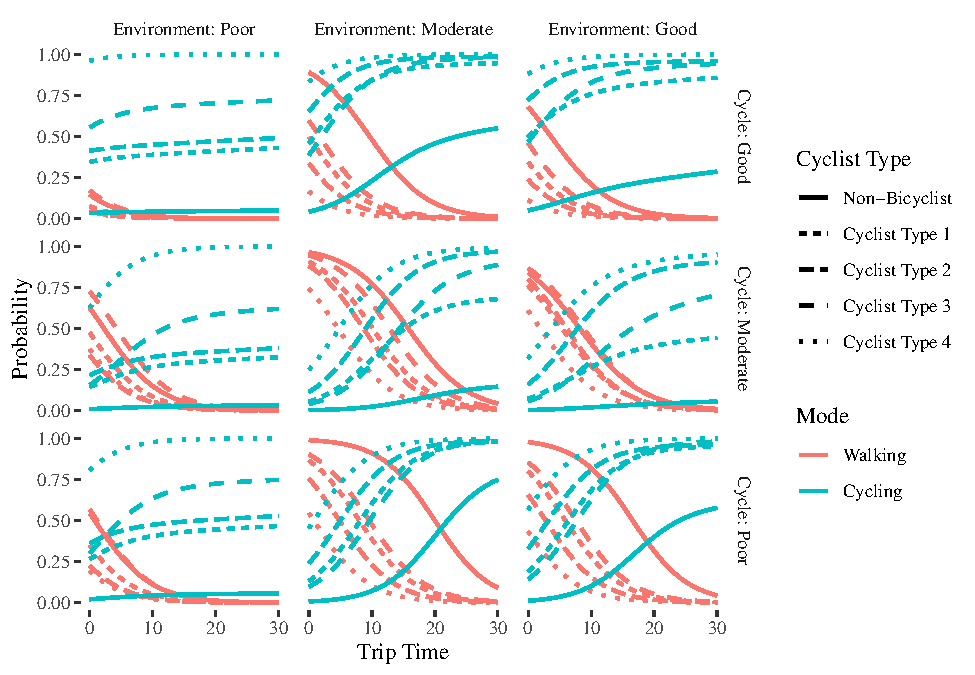
\includegraphics{Active-Travel-in-Bangladesh_files/figure-latex/figure-probabilities-perceptions-active-non-student-residential-1.pdf}
\caption{\label{fig:probabilities-perceptions-active-non-student-residential}Probabilities
of active modes under perceived conditions of the environment in the
neighborhood (crime, conditions for walking, safety from traffic when
walking) vs perceived conditions for cycling, by cycling level of
traveller (non-students in residential land uses).}
\end{figure}

\begin{figure}
\centering
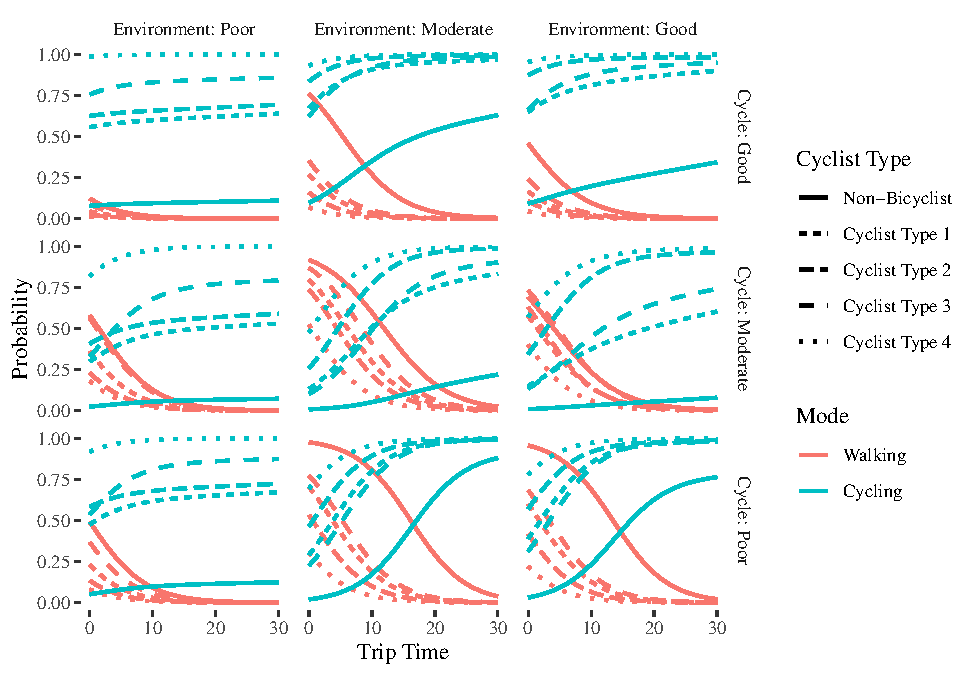
\includegraphics{Active-Travel-in-Bangladesh_files/figure-latex/figure-probabilities-perceptions-active-non-student-non-residential-1.pdf}
\caption{\label{fig:probabilities-perceptions-active-non-student-non-residential}Probabilities
of active modes under perceived conditions of the environment in the
neighborhood (crime, conditions for walking, safety from traffic when
walking) vs perceived conditions for cycling, by cycling level of
traveller (non-students in non-residential land uses).}
\end{figure}

Figure \ref{fig:probabilities-perceptions-active-student-residential}
and Figure
\ref{fig:probabilities-perceptions-active-student-non-residential} show
the simulation for students in residential and non-residential land-use
by perceptions of the environment and perceptions of cycling. Similar to
the non-student population, in both residential and non-residential
land-uses, students' probability of walking for longer duration of
commute increases with the improvement of perceived environmental
conditions and the rate of increase is higher for non-bicyclists
compared to cyclists. Although, after combining the perceived cycling
conditions with other environmental conditions, the probability of
walking for longer commute still increases, the rate of increase is less
compared to the perceived improvements in the environmental conditions.
Probability of cycling for longer duration of commute is higher in the
non-residential land-uses compared to residential land-uses. With the
improvements of perceived environmental conditions as well as perceived
cycling conditions, even student non-bicyclists show a higher
probability of cycling for commute for longer duration in
non-residential land-uses compared to residential land-uses. For
cyclists, improvements in environmental conditions along with cycling
conditions increase the probability of cycling for longer duration of
commute and the rate is higher in non-residential land-uses than in
residential land-uses.

\begin{figure}
\centering
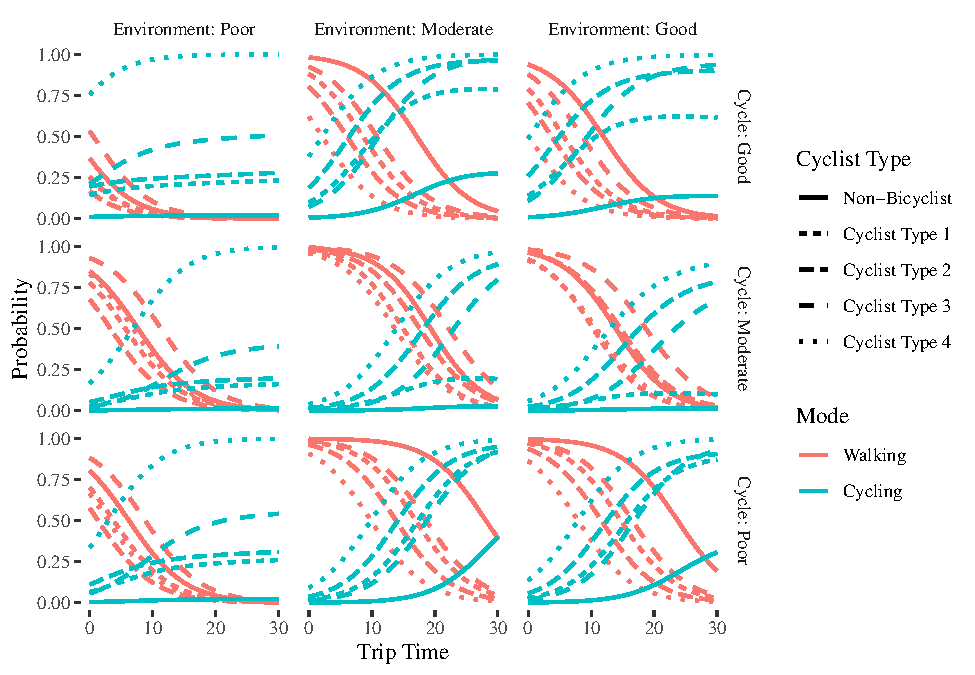
\includegraphics{Active-Travel-in-Bangladesh_files/figure-latex/figure-probabilities-perceptions-active-student-residential-1.pdf}
\caption{\label{fig:probabilities-perceptions-active-student-residential}Probabilities
of active modes under perceived conditions of the environment in the
neighborhood (crime, conditions for walking, safety from traffic when
walking) vs perceived conditions for cycling, by cycling level of
traveller (students in residential land uses).}
\end{figure}

\begin{figure}
\centering
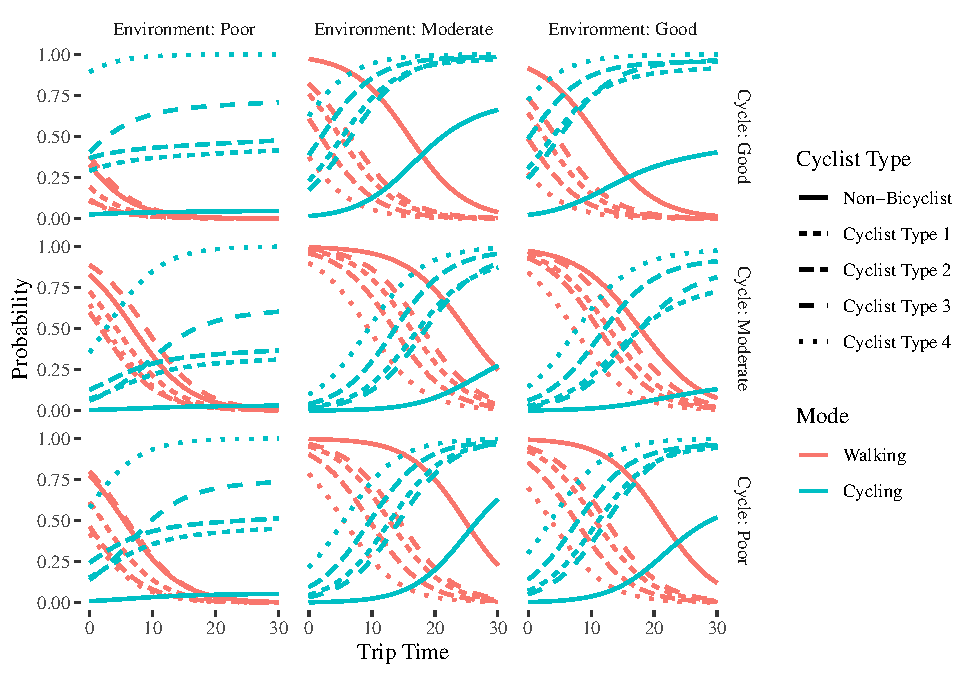
\includegraphics{Active-Travel-in-Bangladesh_files/figure-latex/figure-probabilities-perceptions-active-student-non-residential-1.pdf}
\caption{\label{fig:probabilities-perceptions-active-student-non-residential}Probabilities
of active modes under perceived conditions of the environment in the
neighborhood (crime, conditions for walking, safety from traffic when
walking) vs perceived conditions for cycling, by cycling level of
traveller (students in non-residential land uses).}
\end{figure}

It would be interesting to see what other aspects of the environment
besides cycling conditions contribute to the probability of travel by
active modes. For instance, one might question whether to prioritize
efforts to improve perception of crime or perception of walking
conditions. To explore this, we proceed next to simulate the
probabilities for non-students and students for both residential and
non-residential land-use as follows: we set the perception of cycling to
good, and perceptions of walking (walking and safety while walking) to
poor, moderate, and good. This time, we kept the perceptions of crime
during daytime as a separate variable. We simulate these probabilities
by travel time, ranging from 0-30 min. The number of motorized vehicles
was set to zero.

Figure
\ref{fig:probabilities-perceptions-walking-active-modes-non-students-residential}
and Figure
\ref{fig:probabilities-perceptions-walking-active-modes-non-students-non-residential}
show the simulated probabilities of non-students' active mode use by
perceptions of walking and perceptions of crime as a function of travel
time for residential and non-residential land-use, where perceived
cycling conditions is good. In both land-uses, the probability of
non-bicyclists to use bicycle for longer duration of commute increases
when perceived walking conditions improve from `poor' to `moderate'.
This means that along with `good' cycling conditions, improvement in the
walking condition increases the probability of cycling for commute for
non-bicyclists. For non-student cyclists, improvement in the walking and
crime conditions increases their probability of cycling for longer
duration of commute and the rate is higher in non-residential land-uses
compared to residential land-use. Figure
\ref{fig:probabilities-perceptions-walking-active-modes-students-residential}
and Figure
\ref{fig:probabilities-perceptions-walking-active-modes-students-non-residnetial}
shows the simulation corresponding to students by residential and
non-residential land-use types. A comparison with the preceding figures
indicates that students use active modes more compared to non-students.
With the improvement of walking and crime conditions, the probability of
walking for longer duration of commute increases for non-bicyclists in
both land-use types. The probability of student non-bicyclists of using
bicycle for longer trips increases by improving the walking conditions
in the neighborhood (recall that in this simulation cycling condition is
already set to `good') and the rate of increase is higher in
non-residential land-use compared to residential land-use. For student
cyclists, the probability of using bicycle for longer duration of
commute increases with the improvement of walking and crime conditions
in the neighborhood and the rate of increase is higher in the
non-residential areas compared to residential areas.

\begin{figure}
\centering
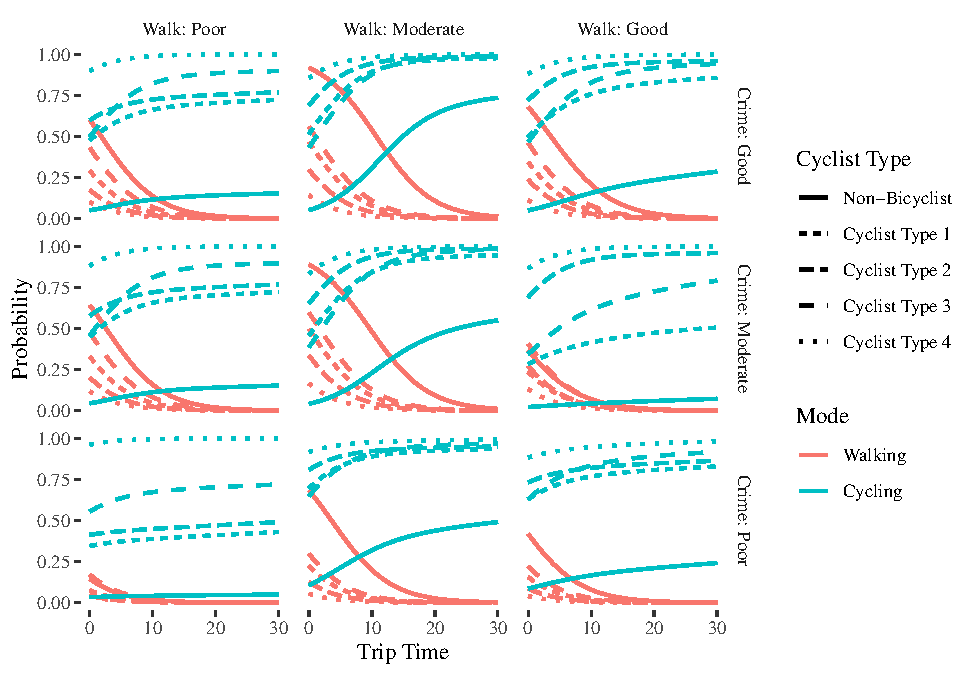
\includegraphics{Active-Travel-in-Bangladesh_files/figure-latex/figure-probabilities-perceptions-walking-active-non-students-residential-1.pdf}
\caption{\label{fig:probabilities-perceptions-walking-active-modes-non-students-residential}Probabilities
of active mode use when perceived conditions for cycling are good:
perceived conditions for walking in the neighborhood (conditions for
walking, safety from traffic when walking) vs perceived crime, by
cycling level of traveller (non-students in residential landuse).}
\end{figure}

\begin{figure}
\centering
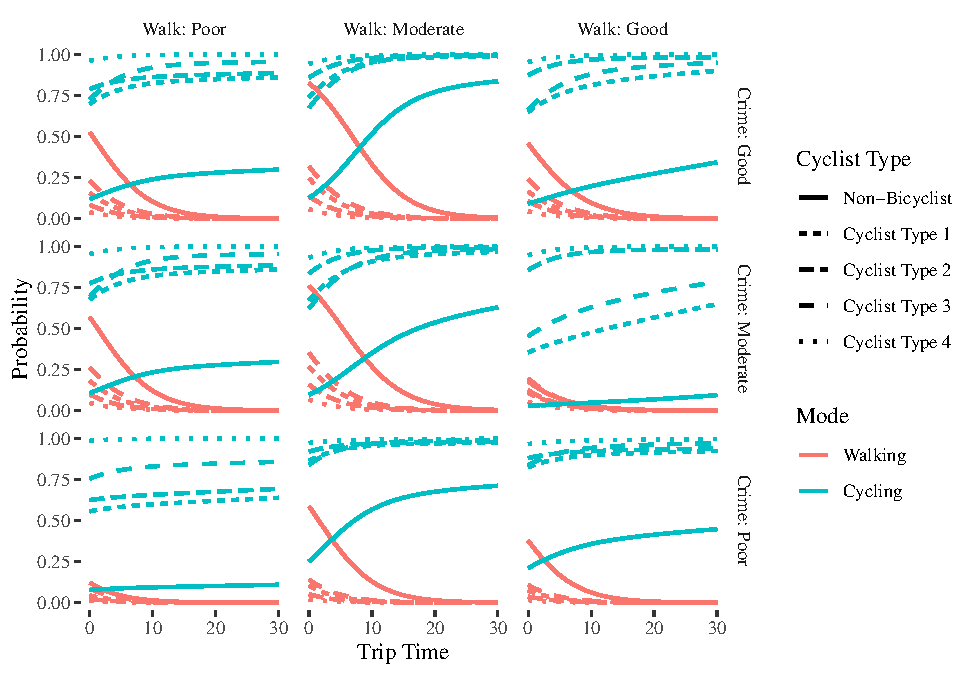
\includegraphics{Active-Travel-in-Bangladesh_files/figure-latex/figure-probabilities-perceptions-walking-active-non-students-non-residential-1.pdf}
\caption{\label{fig:probabilities-perceptions-walking-active-modes-non-students-non-residential}Probabilities
of active mode use when perceived conditions for cycling are good:
perceived conditions for walking in the neighborhood (conditions for
walking, safety from traffic when walking) vs perceived crime, by
cycling level of traveller (non-students in non-residential landuse).}
\end{figure}

\begin{figure}
\centering
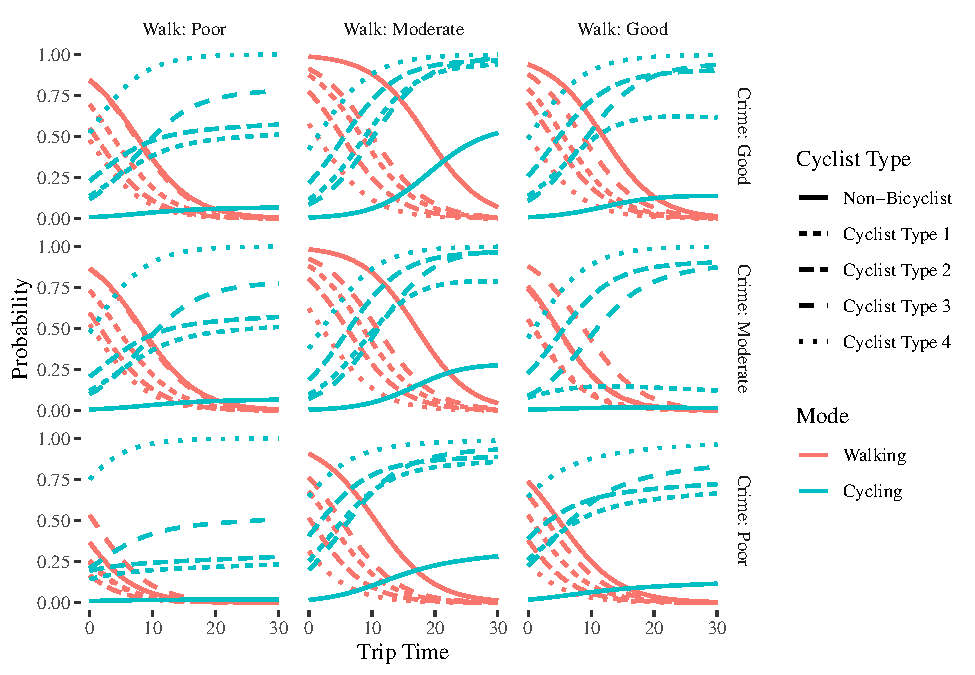
\includegraphics{Active-Travel-in-Bangladesh_files/figure-latex/figure-probabilities-perceptions-walking-active-students-residential-1.pdf}
\caption{\label{fig:probabilities-perceptions-walking-active-modes-students-residential}Probabilities
of active mode use when perceived conditions for cycling are good:
perceived conditions for walking in the neighborhood (conditions for
walking, safety from traffic when walking) vs perceived crime, by
cycling level of traveller (students in residential landuse).}
\end{figure}

\begin{figure}
\centering
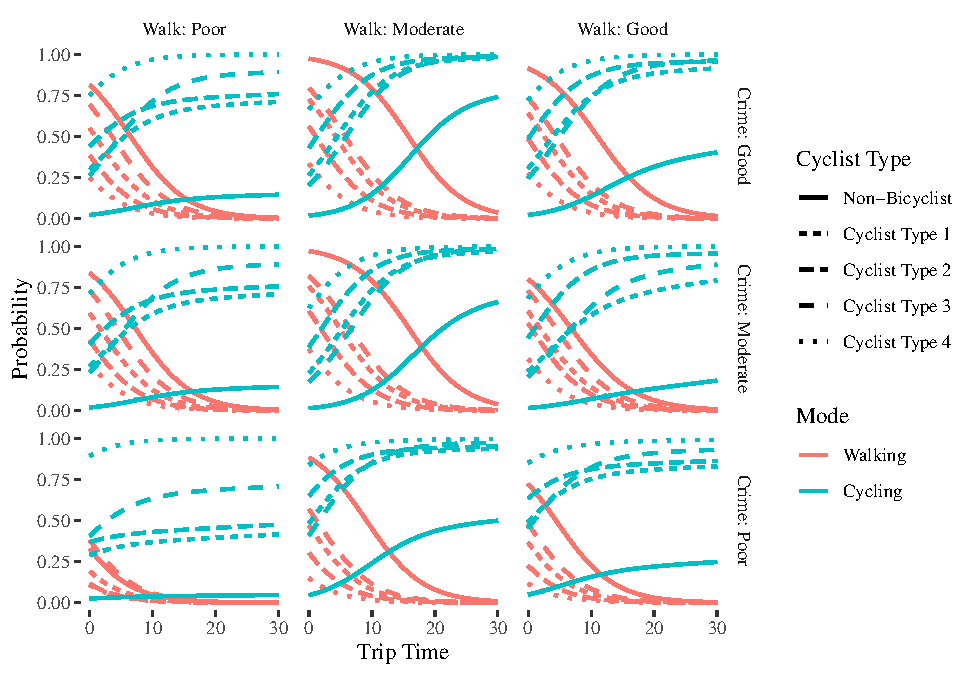
\includegraphics{Active-Travel-in-Bangladesh_files/figure-latex/figure-probabilities-perceptions-walking-active-students-non-residential-1.pdf}
\caption{\label{fig:probabilities-perceptions-walking-active-modes-students-non-residnetial}Probabilities
of active mode use when perceived conditions for cycling are good:
perceived conditions for walking in the neighborhood (conditions for
walking, safety from traffic when walking) vs perceived crime, by
cycling level of traveller (students in non-residential landuse).}
\end{figure}

Figure
\ref{fig:comparison-walk-perceptions-change-non-students-residential}
and Figure
\ref{fig:comparison-walk-perceptions-change-non-students-non-residential}
show the net change in probabilities by active modes for non-students in
residential and non-residential land-uses respectively when perceived
conditions for cycling are good: perceived conditions for walking in the
neighborhood (conditions for walking, safety from traffic when walking)
vs perceived conditions for crime change. In both cases, net increase in
probability of using active modes is higher for non-bicyclist compared
to cyclists, which is expected as cyclists are already cycling daily at
different levels of intensity. For non-student non-bicyclists,
probability of walking for longer duration of commute increases with the
improvement in walking and crime condition in the neighborhood and the
rate is higher in the non-residential land-uses compared to residential
land-uses. On the other hand, their probability of cycling for longer
duration of commute increases when walking conditions is improved from
`poor' to `moderate' and crime conditions from `poor' to `good'.
However, when walking conditions improved from `moderate' to `good' and
with the improvement in the crime conditions, the probabilities of
non-students non-bicyclists' active mode use decreases. One possible
explanation could be that improved neighborhood conditions indicate
affluent neighborhoods, which means that high income households live
there among whom active modes are not popular and they usually use auto
and rickshaw for their daily travel. Similar trend has been noticed for
the student non-bicyclists in Figure
\ref{fig:comparison-walk-perceptions-change-students-residential} and
Figure
\ref{fig:comparison-walk-perceptions-change-students-non-residential}
which show the net change in probabilities by active modes for students
in residential and non-residential land-uses respectively. Additionally,
with improvement in the walking conditions from `poor' to `moderate' and
crime conditions from `poor' to `good', student cyclists tend to use
cycle for longer duration of commute and the rate of increase is higher
compared to student non-bicyclists.

\begin{figure}
\centering
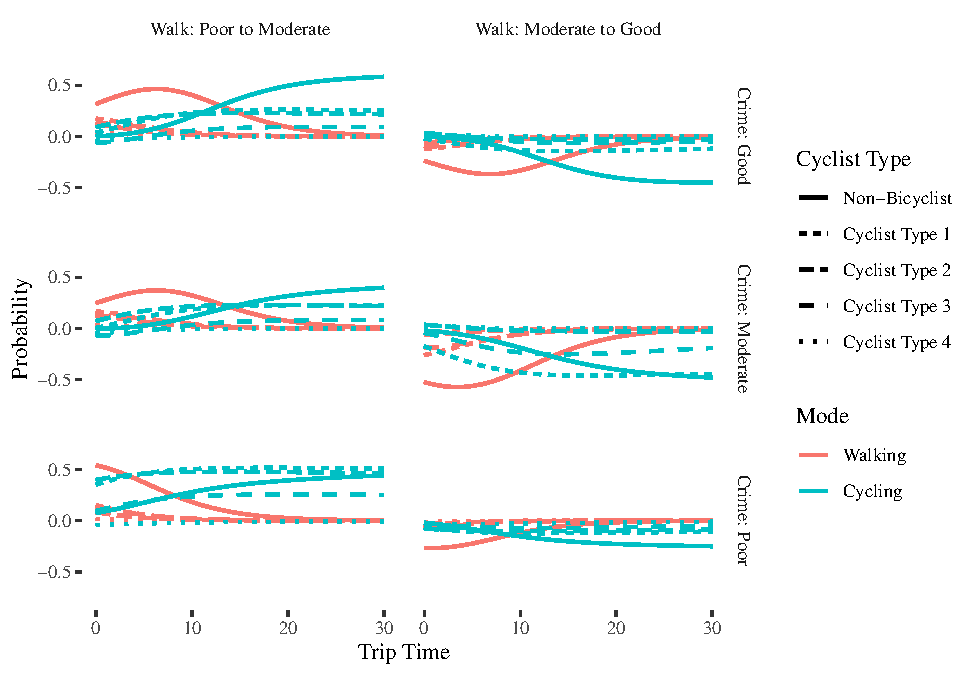
\includegraphics{Active-Travel-in-Bangladesh_files/figure-latex/figure-comparison-walk-perceptions-change-non-students-residential-1.pdf}
\caption{\label{fig:comparison-walk-perceptions-change-non-students-residential}Net
change in probabilities of active mode use when perceived conditions for
cycling are good: perceived conditions for walking in the neighborhood
change (conditions for walking, safety from traffic when walking) vs
perceived crime, by cycling level of traveller (non-students in
residential landuse).}
\end{figure}

\begin{figure}
\centering
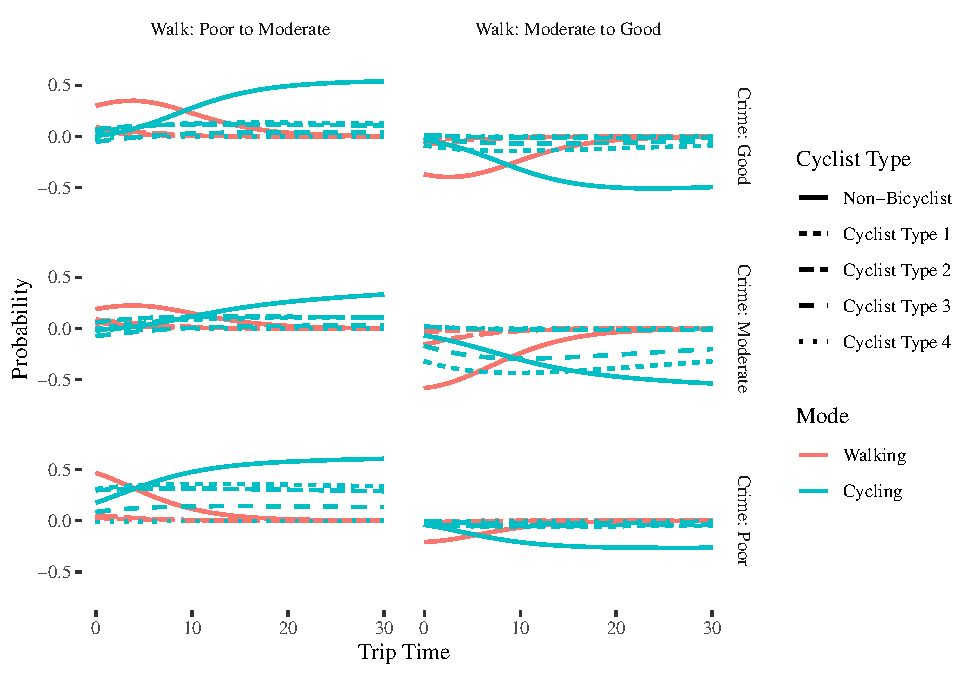
\includegraphics{Active-Travel-in-Bangladesh_files/figure-latex/figure-comparison-walk-perceptions-change-non-students-non-residential-1.pdf}
\caption{\label{fig:comparison-walk-perceptions-change-non-students-non-residential}Net
change in probabilities of active mode use when perceived conditions for
cycling are good: perceived conditions for walking in the neighborhood
change (conditions for walking, safety from traffic when walking) vs
perceived crime, by cycling level of traveller (non-students in
non-residential landuse).}
\end{figure}

\begin{figure}
\centering
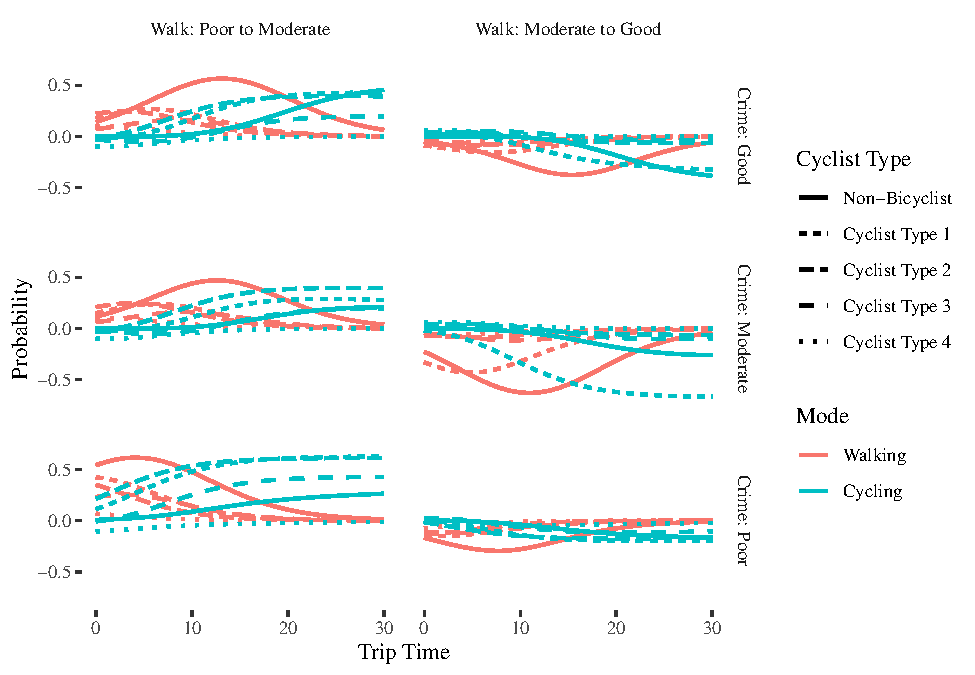
\includegraphics{Active-Travel-in-Bangladesh_files/figure-latex/figure-comparison-walk-perceptions-change-students-residential-1.pdf}
\caption{\label{fig:comparison-walk-perceptions-change-students-residential}Net
change in probabilities of active mode use when perceived conditions for
cycling are good: perceived conditions for walking in the neighborhood
change (conditions for walking, safety from traffic when walking) vs
perceived crime, by cycling level of traveller (students in residential
landuse).}
\end{figure}

\begin{figure}
\centering
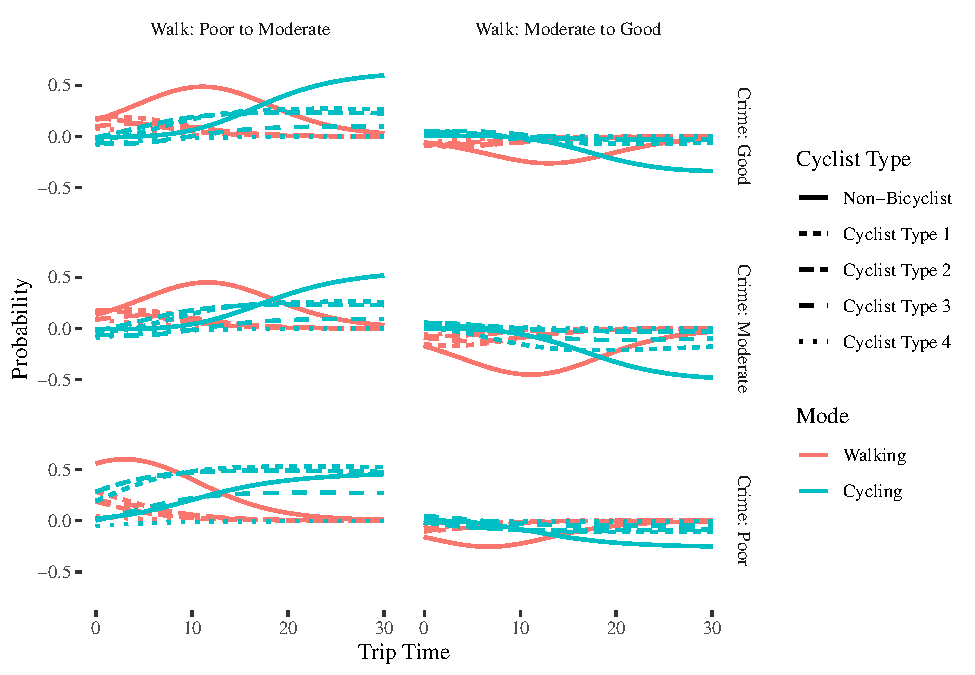
\includegraphics{Active-Travel-in-Bangladesh_files/figure-latex/figure-comparison-walk-perceptions-change-students-non-residential-1.pdf}
\caption{\label{fig:comparison-walk-perceptions-change-students-non-residential}Net
change in probabilities of active mode use when perceived conditions for
cycling are good: perceived conditions for walking in the neighborhood
change (conditions for walking, safety from traffic when walking) vs
perceived crime, by cycling level of traveller (students in
non-residential landuse).}
\end{figure}

Figure
\ref{fig:comparison-crime-perceptions-change-active-non-students-residential}
and Figure
\ref{fig:comparison-crime-perceptions-change-active-non-students-non-residential}
show the net change in probabilities by active modes for non-students in
residential and non-residential land-uses respectively when perceived
conditions for cycling are good: perceived conditions for crime change
vs perceived conditions for walking in the neighborhood (conditions for
walking, safety from traffic when walking). No significant change is
observed in both cases. Figure
\ref{fig:comparison-crime-perceptions-change-active-students-residential}
and Figure
\ref{fig:comparison-crime-perceptions-change-active-students-non-residential}
show the net change in probabilities by active modes for students in
residential and non-residential land-uses respectively when perceived
conditions for cycling are good: perceived conditions for crime change
vs perceived conditions for walking in the neighborhood (conditions for
walking, safety from traffic when walking). For students, probability of
using active modes increases when crime condition in the neighborhood
increases from `poor' to `moderate' and walking condition improves from
`poor' to `moderate' and the change is higher for cyclists compared to
non-cyclists.

\begin{figure}
\centering
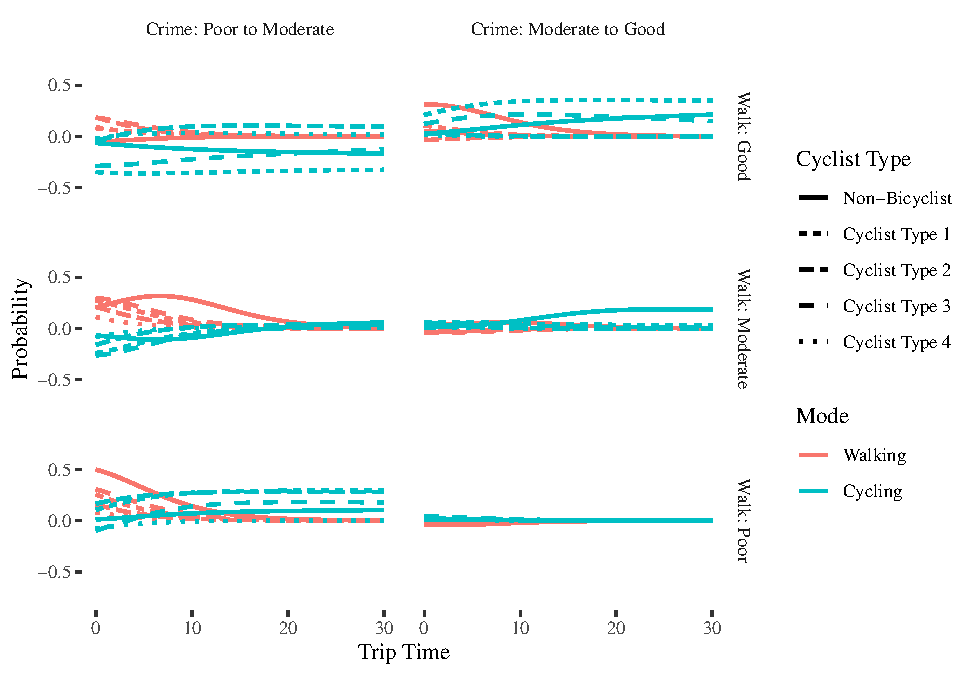
\includegraphics{Active-Travel-in-Bangladesh_files/figure-latex/figure-comparison-crime-perceptions-change-active-non-students-residential-1.pdf}
\caption{\label{fig:comparison-crime-perceptions-change-active-non-students-residential}Net
change in probabilities of active mode use when perceived conditions for
cycling are good: perceived conditions for crime change vs perceived
conditions for walking in the neighborhood (conditions for walking,
safety from traffic when walking), by cycling level of traveller
(non-students in residential land use).}
\end{figure}

\begin{figure}
\centering
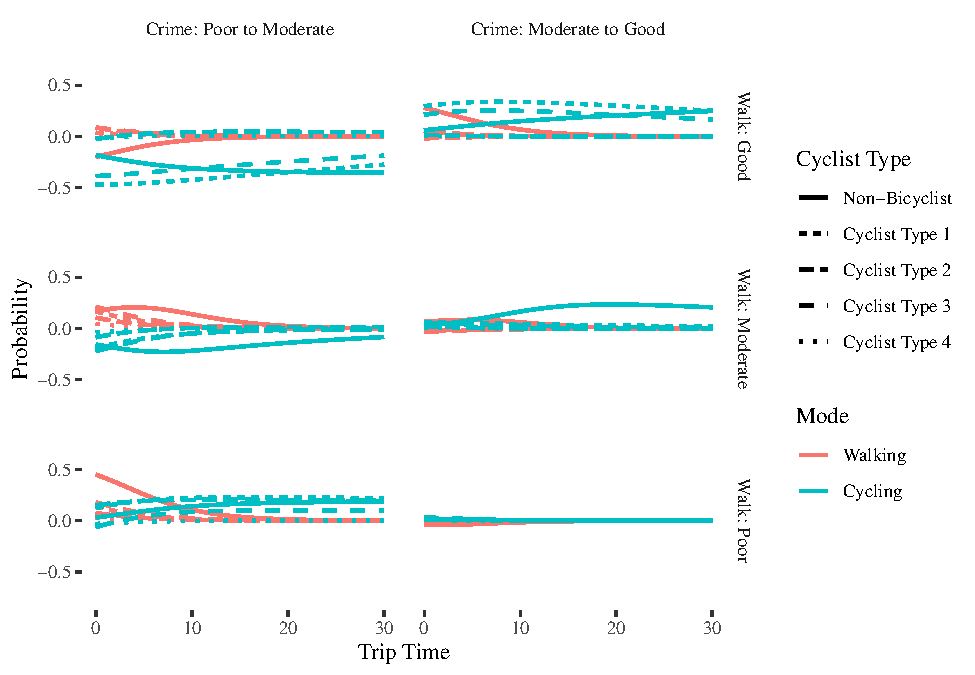
\includegraphics{Active-Travel-in-Bangladesh_files/figure-latex/figure-comparison-crime-perceptions-change-active-non-students-non-residential-1.pdf}
\caption{\label{fig:comparison-crime-perceptions-change-active-non-students-non-residential}Net
change in probabilities of active mode use when perceived conditions for
cycling are good: perceived conditions for crime change vs perceived
conditions for walking in the neighborhood (conditions for walking,
safety from traffic when walking), by cycling level of traveller
(non-students in non-residential land use).}
\end{figure}

\begin{figure}
\centering
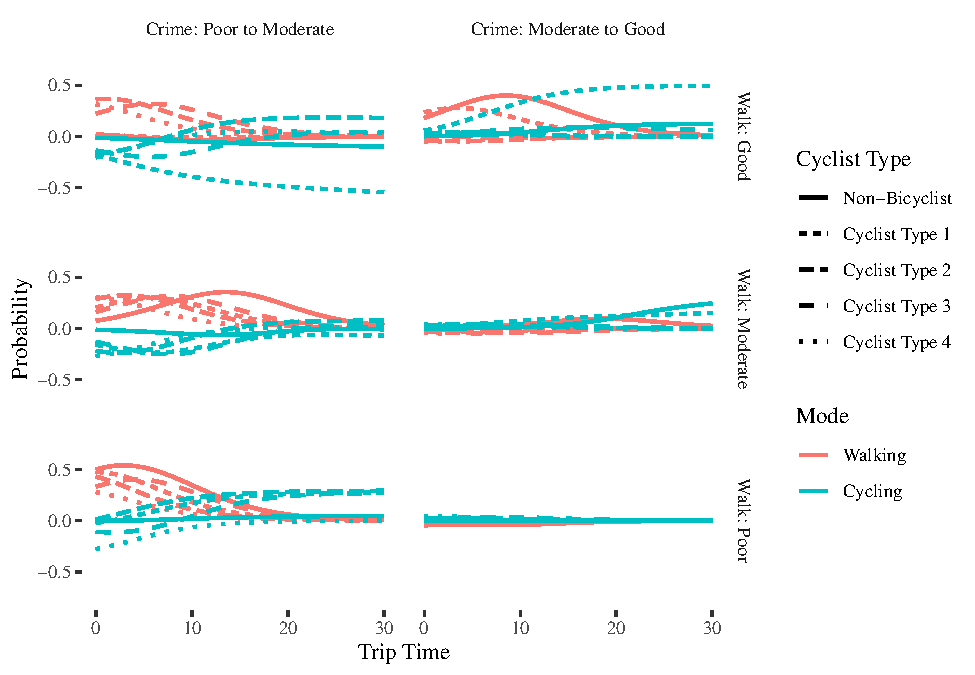
\includegraphics{Active-Travel-in-Bangladesh_files/figure-latex/figure-comparison-crime-perceptions-change-active-students-residential-1.pdf}
\caption{\label{fig:comparison-crime-perceptions-change-active-students-residential}Net
change in probabilities of active mode use when perceived conditions for
cycling are good: perceived conditions for crime change vs perceived
conditions for walking in the neighborhood (conditions for walking,
safety from traffic when walking), by cycling level of traveller
(students in residential land use).}
\end{figure}

\begin{figure}
\centering
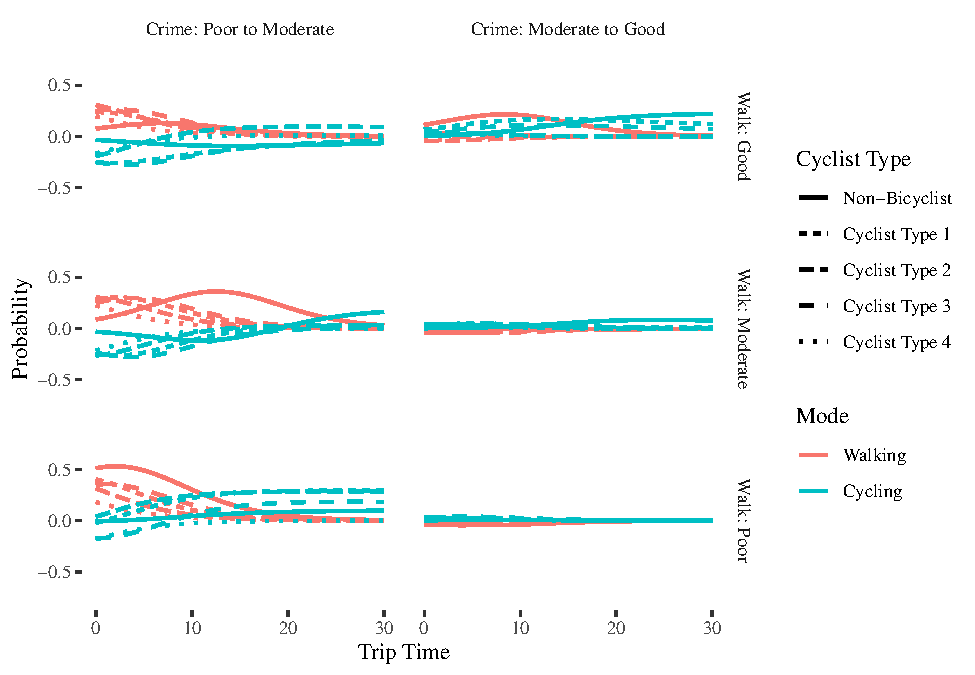
\includegraphics{Active-Travel-in-Bangladesh_files/figure-latex/figure-comparison-crime-perceptions-change-active-students-non-residential-1.pdf}
\caption{\label{fig:comparison-crime-perceptions-change-active-students-non-residential}Net
change in probabilities of active mode use when perceived conditions for
cycling are good: perceived conditions for crime change vs perceived
conditions for walking in the neighborhood (conditions for walking,
safety from traffic when walking), by cycling level of traveller
(students in non-residential land use).}
\end{figure}

\hypertarget{conclusion}{%
\section{Conclusion}\label{conclusion}}

This paper explored the correlates of UAT in the context of a city in
the Global South. The study area was the city of Rajshahi, known as the
Education City of Bangladesh. Along with socio-demographic and trip
characteristics, environmental correlates such as individuals'
perceptions of social (crime and traffic safety) and physical (walking
and cycling) conditions in the neighborhood were studied. To the
authors' best knowledge, this is among the earliest studies that
explored the association between individuals' perceptions and the
probability of traveling by different modes in Rajshahi, Bangladesh. The
study provided an understanding of how travel by active modes is
affected by individual perceptions of the social and physical conditions
in the neighborhood, in addition to individual attributes. There are
differences in socio-cultural contexts between the cities in the Global
South vs.~Global North. Also, socio-cultural contexts within the Global
South cities are different. As there are limited evidence in the context
of the South Asian cities, it is hard to claim that the results of this
study are generalizable to other South Asian cities. More studies in
these areas are needed to reach a concrete conclusion.

The study found that students are more probable users of active modes of
transportation, which is similar to findings reported in developed
countries (e.g., Whalen, Páez, and Carrasco 2013; Molina-García, Sallis,
and Castillo 2014; Delmelle and Delmelle 2012). The results of the study
showed that regular cyclists are more likely to use cycle as a commute
mode compared to non-bicyclists, which indirectly echoes the findings of
Acheampong (2017) and Srinivasan, Pradhan, and Naidu (2007) in the
Global South contexts where they found cycle ownership and higher
frequency of using a cycle increases the likelihood of being an active
commuter. The results of the current study also revealed that the number
of motorized vehicles in the household increases the chance of using
auto or rickshaw for commuting, which is expected in the Bangladeshi
context. In Bangladesh, ownership of a motorized vehicle can be
considered as a proxy for high income (Enam and Choudhury 2011). There
is a fare associated with rickshaw, which makes them comparatively
expensive to UAT modes. Furthermore, rickshaw seems to provide some
reassurance against poor perceptions of crime. Thus, those who own
motorized vehicles are more likely to use auto and rickshaw compared to
UAT modes for their commute. Similar to the findings of Srinivasan,
Pradhan, and Naidu (2007), the study findings indicate that motorized
vehicle ownership discourages active commute. Overall, it can be
concluded from the results that students and individuals with low income
are more likely to use UAT modes compared to other socio-demographic
groups. Thus, policy practitioners should consider initiating programs
to encourage motorized vehicle owners as well as high income groups in
walking and cycling, and/or rewarding active travel in other ways.

This study supports the findings from previous transportation studies
where it has been seen that the probability of walking decreases with
the increase in travel time. However, by assessing the probability of
mode use in different scenarios (i.e.~perceived environmental
conditions), this study revealed that with the increase in the level of
perceptions about the neighborhood conditions, the probability of active
modes, can be increased for longer trips. Non-bicyclists tend to walk
and cyclists tend to cycle for longer duration of commute with the
perceived improvement in the environmental conditions. Non-bicyclists
also show higher probability of using cycle for commute when perceived
environmental conditions are improved. Probability of using cycle for
commute is higher in non-residential land-uses compared to residential
land-uses. Also, simulation of different scenarios suggests that with
the perceived improvements in environmental conditions, students are
more likely to use active modes compared to non-students.

It has been seen that the use of cycle for commuting is more common
among regular cyclists compared to non-bicyclists. The findings show
that the probability of using cycle increases with the improvement of
cycling conditions in the neighborhood. Also, when perceived cycling
condition is good, improvement of perceived walking condition, safety
from traffic and crime conditions in the neighborhood can positively
influence the probability of choosing cycle as a commute mode for longer
duration of travel. Under similar circumstances, the probability of
walking for commute also increases, although the trip duration is less
than cycling. The simulation of different scenarios suggests that the
probability of choosing cycle as a commute mode is more likely to be
increased by improving perceptions of walking conditions from poor to
moderate along with increasing perceived crime conditions. Also, it has
been seen that the rate of increase of probability will be higher for
the improvement of walking conditions (poor to moderate) compared to the
improvement of crime condition. Although non-bicyclists tend to use a
variety of modes for commute, with the improvement of environmental
conditions, cyclists seem to prefer cycle as their commute mode. Policy
implication of this finding is that at first, individuals need to be
encouraged in cycling on a regular basis, which will, therefore,
increase the probability of more people using cycle as a commute mode.
Policies and programs to improve perceptions, such as improving the
condition and ensuring safety from vehicular traffic (e.g.~traffic
signals, traffic calming measures) and crime situations in the
neighborhood can be useful to increase the value of cycling. In the
longer term, perceptions and attitudes can be influenced by developing
and designing walking- and cycling-friendly neighborhoods. For example,
improvement of physical conditions such as development of UAT supportive
infrastructure (e.g.~sidewalks, bike lanes) will increase the
probability of active travel. Also, UAT related promotional activities
could be introduced to address the negative perceptions towards UAT and
creating awareness regarding the benefits of active travel, which is
also proposed by the study of Rosas-Satizábal and Rodriguez-Valencia
(2019) for Bogota, Columbia.

The present study has some limitations that are endemic to studies in
the Global South. First, the study was cross-sectional and not part of a
recurring data collection effort; for this reason, causal effects cannot
be established. Second, detailed data on built-environment
characteristics (say in a GIS) are unavailable for Rajshahi, Bangladesh,
which is why the research used self-reported perceptions by users. Thus,
although previous research has shown that perceptions of the environment
show remarkable geographical consistency (Paez 2013), studying objective
conditions of the built-environment was not possible in this research.
Collecting direct built-environment measures should be emphasized so
that future studies can incorporate them to establish more quantifiable
associations between active modes and environmental factors - thus can
assist the evaluation of the potential impact of built-environment
related interventions on travel by active modes. Micro- or
neighborhood-level data on traffic collisions and crime rates in the
study areas were also unavailable - which can be a scope for future
research. Although it was beyond the scope of the study to collect
information on non-chose modes of commute for the respondents, it would
be interesting to develop a mode choice model with a full choice set
data. The level of service variables for the different modes were not
available for this case study, but should such variables become
available, estimating a latent class choice model would become a new
avenue for research. Future studies could also focus on age-specific and
gender-specific UAT mode use as in developed countries, it has been seen
in other literature that environmental factors affect different age
groups differently (Sallis et al. 2007). Nevertheless, the present study
contributes towards building a better understanding of how perceptions
towards neighborhood level social and physical conditions influence the
use of UAT modes for commuting, which can be used as a basis for
developing travel mode change interventions in the context of Global
South with similar socio-cultural characteristics.

\hypertarget{acknowledgments}{%
\section{Acknowledgments}\label{acknowledgments}}

The authors would like to thank the Bangladesh Institute of Planners for
their `Small Grant for Research' for financial support in this study.
Special thanks are due to the surveyors who completed the field work and
all survey participants. The following \texttt{R} packages were used in
the course of this research, and the authors would like to acknowledge
their developers: \texttt{ggthemes} (Arnold 2019); \texttt{kableExtra}
(Zhu 2019); \texttt{knitr} (Xie 2014, 2015); \texttt{nnet} (Venables and
Ripley 2002); \texttt{pandocfilters} (Schwendinger and Hornik 2019);
\texttt{readxl} (H. Wickham and Bryan 2019); \texttt{reshape2} (Wickham
2007); \texttt{rticles} (Allaire et al. 2020); \texttt{textreg}
(Miratrix 2018); \texttt{tidyverse} (H. Wickham et al. 2019); and
\texttt{tinytex} (Xie 2019, 2020).

\hypertarget{references}{%
\section*{References}\label{references}}
\addcontentsline{toc}{section}{References}

\hypertarget{refs}{}
\leavevmode\hypertarget{ref-acheampong2017towards}{}%
Acheampong, Ransford A. 2017. ``Towards Sustainable Urban Transportation
in Ghana: Exploring Adults' Intention to Adopt Cycling to Work Using
Theory of Planned Behaviour and Structural Equation Modelling.''
\emph{Transportation in Developing Economies} 3 (2): 18.

\leavevmode\hypertarget{ref-adams2010prevalence}{}%
Adams, Jean. 2010. ``Prevalence and Socio-Demographic Correlates of
`Active Transport' in the Uk: Analysis of the Uk Time Use Survey 2005.''
\emph{Preventive Medicine} 50 (4): 199--203.

\leavevmode\hypertarget{ref-adlakha2016neighborhood}{}%
Adlakha, Deepti, J Aaron Hipp, and Ross C Brownson. 2016a.
``Neighborhood-Based Differences in Walkability, Physical Activity, and
Weight Status in India.'' \emph{Journal of Transport \& Health} 3 (4):
485--99.

\leavevmode\hypertarget{ref-adlakha2016adaptation}{}%
Adlakha, Deepti, J Hipp, and Ross Brownson. 2016b. ``Adaptation and
Evaluation of the Neighborhood Environment Walkability Scale in India
(News-India).'' \emph{International Journal of Environmental Research
and Public Health} 13 (4): 401.

\leavevmode\hypertarget{ref-adlakha2018exploring}{}%
Adlakha, Deepti, J Hipp, James Sallis, and Ross Brownson. 2018.
``Exploring Neighborhood Environments and Active Commuting in Chennai,
India.'' \emph{International Journal of Environmental Research and
Public Health} 15 (9): 1840.

\leavevmode\hypertarget{ref-Ajzen1985intentions}{}%
Ajzen, I. 1985. ``From Intentions to Actions: A Theory of Planned
Behavior.'' Book Section. In \emph{Action-Control: From Cognition to
Behavior}, edited by J. Kuhl and J. Beckman, 11--39. Heidelberg:
Springer.

\leavevmode\hypertarget{ref-Akar2009influence}{}%
Akar, Gulsah, and Kelly J Clifton. 2009. ``Influence of Individual
Perceptions and Bicycle Infrastructure on Decision to Bike.'' Journal
Article. \emph{Transportation Research Record} 2140 (1): 165--72.

\leavevmode\hypertarget{ref-Allaire2020rticles}{}%
Allaire, JJ, Yihui Xie, R Foundation, Hadley Wickham, Journal of
Statistical Software, Ramnath Vaidyanathan, Association for Computing
Machinery, et al. 2020. \emph{Rticles: Article Formats for R Markdown}.
\url{https://CRAN.R-project.org/package=rticles}.

\leavevmode\hypertarget{ref-arellana2020urban}{}%
Arellana, Julian, Maria Saltarin, Ana Margarita Larranaga, Vilma
Alvarez, and Cesar Augusto Henao. 2020. ``Urban Walkability Considering
Pedestrians' Perceptions of the Built Environment: A 10-Year Review and
a Case Study in a Medium-Sized City in Latin America.'' \emph{Transport
Reviews} 40 (2): 183--203.

\leavevmode\hypertarget{ref-arellana2020developing}{}%
Arellana, Julian, Maria Saltarin, Ana Margarita Larranaga, Virginia I
Gonzlez, and Cesar Augusto Henao. 2020. ``Developing an Urban
Bikeability Index for Different Types of Cyclists as a Tool to
Prioritise Bicycle Infrastructure Investments.'' \emph{Transportation
Research Part A: Policy and Practice} 139: 310--34.

\leavevmode\hypertarget{ref-arellana2019multivariate}{}%
Arellana, Julián, Luis Fuentes, Joyce Cantillo, and Vilma Alvarez. 2019.
``Multivariate Analysis of User Perceptions About the Serviceability of
Urban Roads: Case of Barranquilla.'' \emph{International Journal of
Pavement Engineering}, 1--10.

\leavevmode\hypertarget{ref-Arnold2019ggthemes}{}%
Arnold, Jeffrey B. 2019. \emph{Ggthemes: Extra Themes, Scales and Geoms
for 'Ggplot2'}. \url{https://CRAN.R-project.org/package=ggthemes}.

\leavevmode\hypertarget{ref-aslam2018cyclability}{}%
Aslam, S Atif Bilal, Houshmand E Masoumi, Muhammad Asim, and Izza Anwer
Minhas. 2018. ``Cyclability in Lahore, Pakistan: Looking into Potential
for Greener Urban Traveling.'' \emph{Tema. Journal of Land Use, Mobility
and Environment} 11 (3): 323--43.

\leavevmode\hypertarget{ref-auckland2016at}{}%
Auckland Transport. 2016. ``Measuring and Growing Active Modes of
Transport in Auckland.''
\url{https://at.govt.nz/media/1957535/at_active-modes-2016.pdf}.

\leavevmode\hypertarget{ref-bangladesh2013raj}{}%
Bangladesh Bureau of Statistics. 2013. ``District Statistics 2011,
Rajshahi.'' Statistics and Information Division, Ministry of Planning.
Government of the People's Republic of Bangladesh.

\leavevmode\hypertarget{ref-bangladesh2015raj}{}%
---------. 2015. ``Population Monograph of Bangladesh. Age-Sex
Composition of Bangladesh Population.'' Statistics and Information
Division, Ministry of Planning. Government of the People's Republic of
Bangladesh.

\leavevmode\hypertarget{ref-Brunsdon2020opening}{}%
Brunsdon, Chris, and Alexis Comber. 2020. ``Opening Practice: Supporting
Reproducibility and Critical Spatial Data Science.'' Journal Article.
\emph{Journal of Geographical Systems}.
\url{https://doi.org/10.1007/s10109-020-00334-2}.

\leavevmode\hypertarget{ref-buehler2011active}{}%
Buehler, Ralph, John Pucher, Dafna Merom, and Adrian Bauman. 2011.
``Active Travel in Germany and the Us: Contributions of Daily Walking
and Cycling to Physical Activity.'' \emph{American Journal of Preventive
Medicine} 41 (3): 241--50.

\leavevmode\hypertarget{ref-Carroll2019modelling}{}%
Carroll, P., B. Caulfield, and A. Ahern. 2019. ``Modelling the Potential
Benefits of Increased Active Travel.'' Journal Article. \emph{Transport
Policy} 79: 82--92. \url{https://doi.org/10.1016/j.tranpol.2019.04.020}.

\leavevmode\hypertarget{ref-cerin2009explaining}{}%
Cerin, Ester, Eva Leslie, and Neville Owen. 2009. ``Explaining
Socio-Economic Status Differences in Walking for Transport: An
Ecological Analysis of Individual, Social and Environmental Factors.''
\emph{Social Science \& Medicine} 68 (6): 1013--20.

\leavevmode\hypertarget{ref-cerin2014ageing}{}%
Cerin, Ester, Cindy HP Sit, Anthony Barnett, Janice M Johnston, Man-Chin
Cheung, and Wai-Man Chan. 2014. ``Ageing in an Ultra-Dense Metropolis:
Perceived Neighbourhood Characteristics and Utilitarian Walking in Hong
Kong Elders.'' \emph{Public Health Nutrition} 17 (1): 225--32.

\leavevmode\hypertarget{ref-cervero2013linking}{}%
Cervero, Robert. 2013. ``Linking Urban Transport and Land Use in
Developing Countries.'' \emph{Journal of Transport and Land Use} 6 (1):
7--24.

\leavevmode\hypertarget{ref-Cervero2014transport}{}%
---------. 2014. ``Transport Infrastructure and the Environment in the
Global South: Sustainable Mobility and Urbanism.'' Journal Article.
\emph{Journal of Regional and City Planning} 25 (3): 174--91.

\leavevmode\hypertarget{ref-Cleland2008perceptions}{}%
Cleland, V. J., A. Timperio, and D. Crawford. 2008. ``Are Perceptions of
the Physical and Social Environment Associated with Mothers' Walking for
Leisure and for Transport? A Longitudinal Study.'' Journal Article.
\emph{Preventive Medicine} 47 (2): 188--93.
\url{ISI:000258560300008\%0Ahttp://ac.els-cdn.com/S0091743508002703/1-s2.0-S0091743508002703-main.pdf?_tid=128949ee-0453-11e7-8058-00000aacb360\&acdnat=1489014229_97f3dd694b9003d735c51e638c70027f}.

\leavevmode\hypertarget{ref-delmelle2012exploring}{}%
Delmelle, Eric M, and Elizabeth Cahill Delmelle. 2012. ``Exploring
Spatio-Temporal Commuting Patterns in a University Environment.''
\emph{Transport Policy} 21: 1--9.

\leavevmode\hypertarget{ref-dill2007factors}{}%
Dill, Jennifer, and Kim Voros. 2007. ``Factors Affecting Bicycling
Demand: Initial Survey Findings from the Portland, Oregon, Region.''
\emph{Transportation Research Record} 2031 (1): 9--17.

\leavevmode\hypertarget{ref-Enam2011methodological}{}%
Enam, Annesha, and Charisma F Choudhury. 2011. ``Methodological Issues
in Developing Mode Choice Models for Dhaka, Bangladesh.''
\emph{Transportation Research Record} 2239 (1): 84--92.

\leavevmode\hypertarget{ref-Gatersleben2007contemplating}{}%
Gatersleben, B., and K. M. Appleton. 2007. ``Contemplating Cycling to
Work: Attitudes and Perceptions in Different Stages of Change.'' Journal
Article. \emph{Transportation Research Part A-Policy and Practice} 41
(4): 302--12. \url{https://doi.org/10.1016/j.tra.2006.09.002}.

\leavevmode\hypertarget{ref-giles2002socioeconomic}{}%
Giles-Corti, Billie, and Robert J Donovan. 2002. ``Socioeconomic Status
Differences in Recreational Physical Activity Levels and Real and
Perceived Access to a Supportive Physical Environment.''
\emph{Preventive Medicine} 35 (6): 601--11.

\leavevmode\hypertarget{ref-godefrooij2010co}{}%
Godefrooij, T, and S Schepel. 2010. ``Co-Benefits of Cycling-Inclusive
Planning and Promotion.'' \emph{World Bank, Netherlands}.

\leavevmode\hypertarget{ref-gomes2011walking}{}%
Gomes, Grace AO, Rodrigo S Reis, Diana C Parra, Isabela Ribeiro, Adriano
AF Hino, Pedro C Hallal, Deborah C Malta, and Ross C Brownson. 2011.
``Walking for Leisure Among Adults from Three Brazilian Cities and Its
Association with Perceived Environment Attributes and Personal
Factors.'' \emph{International Journal of Behavioral Nutrition and
Physical Activity} 8 (1): 111.

\leavevmode\hypertarget{ref-bangla2013policy}{}%
Government of Bangladesh. 2013. ``National Integrated Multimodal
Transport Policy.'' Government of the People's Republic of Bangladesh.

\leavevmode\hypertarget{ref-gomez2010built}{}%
Gómez, Luis F, Diana C Parra, David Buchner, Ross C Brownson, Olga L
Sarmiento, José D Pinzón, Mauricio Ardila, José Moreno, Mauricio
Serrato, and Felipe Lobelo. 2010. ``Built Environment Attributes and
Walking Patterns Among the Elderly Population in Bogotá.''
\emph{American Journal of Preventive Medicine} 38 (6): 592--99.

\leavevmode\hypertarget{ref-Grosse2018exploring}{}%
Grosse, J., A. S. Olafsson, T. A. Carstensen, and C. Fertner. 2018.
``Exploring the Role of Daily "Modality Styles" and Urban Structure in
Holidays and Longer Weekend Trips: Travel Behaviour of Urban and
Peri-Urban Residents in Greater Copenhagen.'' Journal Article.
\emph{Journal of Transport Geography} 69: 138--49.
\url{https://doi.org/10.1016/j.jtrangeo.2018.04.008}.

\leavevmode\hypertarget{ref-gul2018association}{}%
Gul, Yasmeen, Zahid Sultan, and Gul Ahmed Jokhio. 2018. ``The
Association Between the Perception of Crime and Walking in Gated and
Non-Gated Neighbourhoods of Asian Developing Countries.'' \emph{Heliyon}
4 (8): e00715.

\leavevmode\hypertarget{ref-gutierrez2020estimating}{}%
Gutirrez, Margareth, Victor Cantillo, Julian Arellana, and Juan de Dios
Ortuzar. 2020. ``Estimating Bicycle Demand in an Aggressive
Environment.'' \emph{International Journal of Sustainable
Transportation}, 1--14.

\leavevmode\hypertarget{ref-guzman2020confronting}{}%
Guzman, Luis A, Julian Arellana, and Vilma Alvarez. 2020. ``Confronting
Congestion in Urban Areas: Developing Sustainable Mobility Plans for
Public and Private Organizations in Bogotá.'' \emph{Transportation
Research Part A: Policy and Practice} 134: 321--35.

\leavevmode\hypertarget{ref-gwilliam2003urban}{}%
Gwilliam, Ken. 2003. ``Urban Transport in Developing Countries.''
\emph{Transport Reviews} 23 (2): 197--216.

\leavevmode\hypertarget{ref-gwilliam2013cities}{}%
Gwilliam, Kenneth. 2013. ``Cities on the Move--Ten Years After.''
\emph{Research in Transportation Economics} 40 (1): 3--18.

\leavevmode\hypertarget{ref-hallal2010association}{}%
Hallal, Pedro C, Rodrigo S Reis, Diana C Parra, Christine Hoehner, Ross
C Brownson, and Eduardo J Simões. 2010. ``Association Between Perceived
Environmental Attributes and Physical Activity Among Adults in Recife,
Brazil.'' \emph{Journal of Physical Activity and Health} 7 (s2):
S213--S222.

\leavevmode\hypertarget{ref-hammadi_2016}{}%
Hammadi, Saad. 2016. ``Rajshahi: The City That Took on Air Pollution and
Won.'' \emph{The Guardian}, June.
\url{https://www.theguardian.com/world/2016/jun/17/rajshahi-bangladesh-city-air-pollution-won}.

\leavevmode\hypertarget{ref-haque2014}{}%
Haque, Ashraful. 2014. ``Transport Situation in Rajshahi.'' Presenetd at
the United Nations Economic; Social Commission for Asia; the Pacific (UN
ESCAP)".

\leavevmode\hypertarget{ref-hatamzadeh2017walking}{}%
Hatamzadeh, Yaser, Meeghat Habibian, and Ali Khodaii. 2017. ``Walking
and Jobs: A Comparative Analysis to Explore Factors Influencing Flexible
and Fixed Schedule Workers, a Case Study of Rasht, Iran.''
\emph{Sustainable Cities and Society} 31: 74--82.

\leavevmode\hypertarget{ref-hossain_2018}{}%
Hossain, Iqbal. 2018. ``Women Labour Force in Bangladesh: Key Facts and
Trends.'' \emph{The Financial Express}.
\url{https://today.thefinancialexpress.com.bd/26th-anniversary-issue-3/women-labour-force-in-bangladesh-key-facts-and-trends-1544443424}.

\leavevmode\hypertarget{ref-huertas2020level}{}%
Huertas, Jorge A, Alejandro Palacio, Marcelo Botero, Germán A Carvajal,
Thomas van Laake, Diana Higuera-Mendieta, Sergio A Cabrales, Luis A
Guzman, Olga L Sarmiento, and Andrés L Medaglia. 2020. ``Level of
Traffic Stress-Based Classification: A Clustering Approach for Bogotá,
Colombia.'' \emph{Transportation Research Part D: Transport and
Environment} 85: 102420.

\leavevmode\hypertarget{ref-Jamal2020}{}%
Jamal, Shaila., and Mohiuddin Hossain. 2020. ``Active Transportation
Indicators and Establishing Baseline in a Developing Country Context: A
Study of Rajshahi, Bangladesh.'' Journal Article. \emph{Growth and
Change - A Journal of Urban and Regional Policy}.
\href{https://doi.org/DOI:\%2010.1111/grow.12420\%20}{https://doi.org/DOI: 10.1111/grow.12420}.

\leavevmode\hypertarget{ref-Jappinen2013modelling}{}%
Jäppinen, Sakari, Tuuli Toivonen, and Maria Salonen. 2013. ``Modelling
the Potential Effect of Shared Bicycles on Public Transport Travel Times
in Greater Helsinki: An Open Data Approach.'' Journal Article.
\emph{Applied Geography} 43: 13--24.

\leavevmode\hypertarget{ref-jia2014association}{}%
Jia, Yingnan, Tricia Usagawa, and Hua Fu. 2014. ``The Association
Between Walking and Perceived Environment in Chinese Community
Residents: A Cross-Sectional Study.'' \emph{PloS One} 9 (2): e90078.

\leavevmode\hypertarget{ref-khan_2017}{}%
Khan, Maliha. 2017. ``Rajshahi: A Model for Tackling Ambient Air
Pollution in Our Cities.'' \emph{The Daily Star}, June.
\url{https://www.thedailystar.net/star-weekend/rajshahi-model-tackling-ambient-air-pollution-our-cities-1414174}.

\leavevmode\hypertarget{ref-Korzhenevych2018area}{}%
Korzhenevych, A., and M. Jain. 2018. ``Area- and Gender-Based Commuting
Differentials in India's Largest Urban-Rural Region.'' Journal Article.
\emph{Transportation Research Part D-Transport and Environment} 63:
733--46. \url{https://doi.org/10.1016/j.trd.2018.07.013}.

\leavevmode\hypertarget{ref-Krueger2018normative}{}%
Krueger, R., A. Vij, and T. H. Rashidi. 2018. ``Normative Beliefs and
Modality Styles: A Latent Class and Latent Variable Model of Travel
Behaviour.'' Journal Article. \emph{Transportation} 45 (3): 789--825.
\url{https://doi.org/10.1007/s11116-016-9751-1}.

\leavevmode\hypertarget{ref-kuranami1994factors}{}%
Kuranami, Chiaki, and Bruce P Winston. 1994. ``Factors Influencing
Ownership and Use of Nonmotorized Vehicles in Asian Cities.''
\emph{Transportation Research Record}, no. 1441.

\leavevmode\hypertarget{ref-Landman2012crime}{}%
Landman, Karina. 2012. ``Reconsidering Crime and Urban Fortification in
South Africa.'' Book Section. In \emph{The Urban Fabric of Crime and
Fear}, edited by Vania Ceccato, 239--64. Dordrecht: Springer
Netherlands. \url{https://doi.org/10.1007/978-94-007-4210-9_10}.

\leavevmode\hypertarget{ref-larranaga2019using}{}%
Larranaga, Ana Margarita, Julián Arellana, Luis Ignacio Rizzi, Orlando
Strambi, and Helena Beatriz Bettella Cybis. 2019. ``Using Best--Worst
Scaling to Identify Barriers to Walkability: A Study of Porto Alegre,
Brazil.'' \emph{Transportation} 46 (6): 2347--79.

\leavevmode\hypertarget{ref-larranaga2016influence}{}%
Larrañaga, Ana Margarita, Luis Ignacio Rizzi, Julian Arellana, Orlando
Strambi, and Helena Beatriz Bettella Cybis. 2016. ``The Influence of
Built Environment and Travel Attitudes on Walking: A Case Study of Porto
Alegre, Brazil.'' \emph{International Journal of Sustainable
Transportation} 10 (4): 332--42.

\leavevmode\hypertarget{ref-laverty2013active}{}%
Laverty, Anthony A, Jennifer S Mindell, Elizabeth A Webb, and
Christopher Millett. 2013. ``Active Travel to Work and Cardiovascular
Risk Factors in the United Kingdom.'' \emph{American Journal of
Preventive Medicine} 45 (3): 282--88.

\leavevmode\hypertarget{ref-Lavery2013driving}{}%
Lavery, T. A., A. Paez, and P. S. Kanaroglou. 2013. ``Driving Out of
Choices: An Investigation of Transport Modality in a University
Sample.'' Journal Article. \emph{Transportation Research Part A-Policy
and Practice} 57: 37--46.
\url{https://doi.org/10.1016/j.tra.2013.09.010}.

\leavevmode\hypertarget{ref-Lemanski2012everyday}{}%
Lemanski, C. 2012. ``Everyday Human (in)security: Rescaling for the
Southern City.'' Journal Article. \emph{Security Dialogue} 43 (1):
61--78. \url{https://doi.org/10.1177/0967010611430435}.

\leavevmode\hypertarget{ref-Li2011decoupling}{}%
Li, Jun. 2011. ``Decoupling Urban Transport from Ghg Emissions in Indian
Cities-a Critical Review and Perspectives.'' Journal Article.
\emph{Energy Policy} 39 (6): 3503--14.
\url{https://doi.org/10.1016/j.enpol.2011.03.049}.

\leavevmode\hypertarget{ref-liao2015perceived}{}%
Liao, Yung, I Wang, Hsiu-Hua Hsu, Shao-Hsi Chang, and others. 2015.
``Perceived Environmental and Personal Factors Associated with Walking
and Cycling for Transportation in Taiwanese Adults.''
\emph{International Journal of Environmental Research and Public Health}
12 (2): 2105--19.

\leavevmode\hypertarget{ref-Loo2015transport}{}%
Loo, L. Y. L., J. Corcoran, D. Mateo-Babiano, and R. Zahnow. 2015.
``Transport Mode Choice in South East Asia: Investigating the
Relationship Between Transport Users' Perception and Travel Behaviour in
Johor Bahru, Malaysia.'' Journal Article. \emph{Journal of Transport
Geography} 46: 99--111.
\url{https://doi.org/10.1016/j.jtrangeo.2015.06.011}.

\leavevmode\hypertarget{ref-mackenbach2016influence}{}%
Mackenbach, Joreintje, Edward Randal, Pengjun Zhao, and Philippa
Howden-Chapman. 2016. ``The Influence of Urban Land-Use and Public
Transport Facilities on Active Commuting in Wellington, New Zealand:
Active Transport Forecasting Using the Wilute Model.''
\emph{Sustainability} 8 (3): 242.

\leavevmode\hypertarget{ref-Martin2014active}{}%
Martin, A., Y. Goryakin, and M. Suhrcke. 2014. ``Does Active Commuting
Improve Psychological Wellbeing? Longitudinal Evidence from Eighteen
Waves of the British Household Panel Survey.'' Journal Article.
\emph{Preventive Medicine} 69: 296--303.
\url{https://doi.org/10.1016/j.ypmed.2014.08.023}.

\leavevmode\hypertarget{ref-Martin2019individual}{}%
Martín, Belén, and Antonio Páez. 2019. ``Individual and Geographic
Variations in the Propensity to Travel by Active Modes in
Vitoria-Gasteiz, Spain.'' Journal Article. \emph{Journal of Transport
Geography} 76: 103--13.
\url{https://doi.org/https://doi.org/10.1016/j.jtrangeo.2019.03.005}.

\leavevmode\hypertarget{ref-Miller2011collaborative}{}%
Miller, Harvey J. 2011. ``Collaborative Mobility: Using Geographic
Information Science to Cultivate Cooperative Transportation Systems.''
Journal Article. \emph{Procedia - Social and Behavioral Sciences} 21
(0): 24--28.
\url{https://doi.org/http://dx.doi.org/10.1016/j.sbspro.2011.07.005}.

\leavevmode\hypertarget{ref-Miratrix2018textreg}{}%
Miratrix, Luke. 2018. \emph{Textreg: N-Gram Text Regression, Aka Concise
Comparative Summarization}.
\url{https://CRAN.R-project.org/package=textreg}.

\leavevmode\hypertarget{ref-mitra2016}{}%
Mitra, Suman Kumar. 2016. ``Land Use, Land Value, and Transportation:
Essays on Accessibility, Carless Households, and Long-Distance Travel.''
PhD thesis, University of California, Irvine.

\leavevmode\hypertarget{ref-molina2014active}{}%
Molina-García, Javier, James F Sallis, and Isabel Castillo. 2014.
``Active Commuting and Sociodemographic Factors Among University
Students in Spain.'' \emph{Journal of Physical Activity and Health} 11
(2): 359--63.

\leavevmode\hypertarget{ref-Moniruzzaman2012model}{}%
Moniruzzaman, M., and A. Paez. 2012. ``A Model-Based Approach to Select
Case Sites for Walkability Audits.'' Journal Article. \emph{Health \&
Place} 18 (6): 1323--34.
\url{https://doi.org/10.1016/j.healthplace.2012.09.013}.

\leavevmode\hypertarget{ref-Moniruzzaman2016investigation}{}%
---------. 2016. ``An Investigation of the Attributes of Walkable
Environments from the Perspective of Seniors in Montreal.'' Journal
Article. \emph{Journal of Transport Geography} 51: 85--96.
\url{https://doi.org/10.1016/j.jtrangeo.2015.12.001}.

\leavevmode\hypertarget{ref-Moniruzzaman2014compliance}{}%
Moniruzzaman, M., A. Paez, and C. Morency. 2014. ``Compliance Potential
Mapping: A Tool to Assess Potential Contributions of Walking Towards
Physical Activity Guidelines.'' Journal Article. \emph{BMC Public
Health} 14: 11. \url{https://doi.org/10.1186/1471-2458-14-511}.

\leavevmode\hypertarget{ref-de2012association}{}%
Munter, Jeroen SL de, Charles Agyemang, Lizzy M Brewster, Karien
Stronks, and Irene GM van Valkengoed. 2012. ``The Association of
Leisure-Time Physical Activity and Active Commuting with Measures of
Socioeconomic Position in a Multiethnic Population Living in the
Netherlands: Results from the Cross-Sectional Sunset Study.'' \emph{BMC
Public Health} 12 (1): 815.

\leavevmode\hypertarget{ref-deNazelle2011improving}{}%
Nazelle, A. de, M. J. Nieuwenhuijsen, J. M. Anto, M. Brauer, D. Briggs,
C. Braun-Fahrlander, N. Cavill, et al. 2011. ``Improving Health Through
Policies That Promote Active Travel: A Review of Evidence to Support
Integrated Health Impact Assessment.'' Journal Article.
\emph{Environment International} 37 (4): 766--77.
\url{https://doi.org/10.1016/j.envint.2011.02.003}.

\leavevmode\hypertarget{ref-Nobis2007multimodality}{}%
Nobis, C. 2007. ``Multimodality - Facets and Causes of Sustainable
Mobility Behavior.'' Journal Article. \emph{Transportation Research
Record}, no. 2010: 37--46. \url{ISI:000252769600005}.

\leavevmode\hypertarget{ref-oliva2018identifying}{}%
Oliva, Ignacio, Patricia Galilea, and Ricardo Hurtubia. 2018.
``Identifying Cycling-Inducing Neighborhoods: A Latent Class Approach.''
\emph{International Journal of Sustainable Transportation} 12 (10):
701--13.

\leavevmode\hypertarget{ref-oyeyemi2012perceived}{}%
Oyeyemi, Adewale L, Babatunde O Adegoke, James F Sallis, Adetoyeje Y
Oyeyemi, and Ilse De Bourdeaudhuij. 2012. ``Perceived Crime and Traffic
Safety Is Related to Physical Activity Among Adults in Nigeria.''
\emph{BMC Public Health} 12 (1): 294.

\leavevmode\hypertarget{ref-Paez2013mapping}{}%
Paez, A. 2013. ``Mapping Travelers' Attitudes: Does Space Matter?''
Journal Article. \emph{Journal of Transport Geography} 26: 117--25.
\url{https://doi.org/10.1016/j.jtrangeo.2012.09.002}.

\leavevmode\hypertarget{ref-parra2011perceived}{}%
Parra, Diana C, Christine M Hoehner, Pedro C Hallal, Isabela C Ribeiro,
Rodrigo Reis, Ross C Brownson, Michael Pratt, and Eduardo J Simoes.
2011. ``Perceived Environmental Correlates of Physical Activity for
Leisure and Transportation in Curitiba, Brazil.'' \emph{Preventive
Medicine} 52 (3-4): 234--38.

\leavevmode\hypertarget{ref-peterborough2014at}{}%
Peterborough City and County. 2014. ``Active Transport and Health
Indicators Report.''
\url{http://peterboroughmoves.com/wp-content/uploads/2015/05/IndicatorsReport_Final_Web.pdf}.

\leavevmode\hypertarget{ref-pojani2015sustainable}{}%
Pojani, Dorina, and Dominic Stead. 2015. ``Sustainable Urban Transport
in the Developing World: Beyond Megacities.'' \emph{Sustainability} 7
(6): 7784--7805.

\leavevmode\hypertarget{ref-poushter_2015}{}%
Poushter, Jacob. 2015. ``Car, Bike or Motorcycle? Depends on Where You
Live.'' \emph{Pew Research Center}. Pew Research Center.
\url{https://www.pewresearch.org/fact-tank/2015/04/16/car-bike-or-motorcycle-depends-on-where-you-live/}.

\leavevmode\hypertarget{ref-power2016bd}{}%
Power and Participation Research Centre. 2016. ``Bangladesh 2016:
Politics, Governance and Middle Income Aspirations: Realities and
Challenges: An Empirical Study.''
\url{https://www.undp.org/content/dam/bangladesh/docs/Publications/Pub2016/policy\%20brief.pdf}.

\leavevmode\hypertarget{ref-public2011can}{}%
Public Health Agency of Canada. 2011. ``Fast Facts About Canada's
Neighborhoods and Physical Activity. Data Compiled from the 2011
Canadian Community Health Survey Rapid Response Module on Neighborhood
Environments.''
\url{https://www.canada.ca/content/dam/phac-aspc/migration/phac-aspc/hp-ps/hl-mvs/assets/pdf/fast-facts-faits-rapidesV2-eng.pdf}.

\leavevmode\hypertarget{ref-pucher2011walking}{}%
Pucher, John, Ralph Buehler, Dafna Merom, and Adrian Bauman. 2011.
``Walking and Cycling in the United States, 2001--2009: Evidence from
the National Household Travel Surveys.'' \emph{American Journal of
Public Health} 101 (S1): S310--S317.

\leavevmode\hypertarget{ref-rahul2013economic}{}%
Rahul, TM, and Ashish Verma. 2013. ``Economic Impact of Non-Motorized
Transportation in Indian Cities.'' \emph{Research in Transportation
Economics} 38 (1): 22--34.

\leavevmode\hypertarget{ref-rosas2019factors}{}%
Rosas-Satizábal, Daniel, and Alvaro Rodriguez-Valencia. 2019. ``Factors
and Policies Explaining the Emergence of the Bicycle Commuter in
Bogotá.'' \emph{Case Studies on Transport Policy} 7 (1): 138--49.

\leavevmode\hypertarget{ref-rossetti2019want}{}%
Rossetti, Tomás, Verónica Saud, and Ricardo Hurtubia. 2019. ``I Want to
Ride It Where I Like: Measuring Design Preferences in Cycling
Infrastructure.'' \emph{Transportation}, 1--22.

\leavevmode\hypertarget{ref-sallis2007perceived}{}%
Sallis, James F, Abby C King, John R Sirard, and Cheryl L Albright.
2007. ``Perceived Environmental Predictors of Physical Activity over 6
Months in Adults: Activity Counseling Trial.'' \emph{Health Psychology}
26 (6): 701.

\leavevmode\hypertarget{ref-sa2016socioeconomic}{}%
Sá, Thiago Hérick de, Rafael Henrique Moraes Pereira, Ana Clara Duran,
and Carlos Augusto Monteiro. 2016. ``Socioeconomic and Regional
Differences in Active Transportation in Brazil.'' \emph{Revista de Saude
Publica} 50: 37.

\leavevmode\hypertarget{ref-sa2016cycling}{}%
Sá, Thiago Hérick, Ana Clara Duran, Marko Tainio, Carlos Augusto
Monteiro, and James Woodcock. 2016. ``Cycling in São Paulo, Brazil
(1997--2012): Correlates, Time Trends and Health Consequences.''
\emph{Preventive Medicine Reports} 4: 540--45.

\leavevmode\hypertarget{ref-Schwendinger2019pandocfilters}{}%
Schwendinger, Florian, and Kurt Hornik. 2019. \emph{Pandocfilters:
Pandoc Filters for R}.
\url{https://CRAN.R-project.org/package=pandocfilters}.

\leavevmode\hypertarget{ref-da2017factors}{}%
Silva Bandeira, Alexsandra da, Kelly Samara da Silva, Giovâni Firpo Del
Duca, Geyson Ricardo Zilch, Elusa Santina Antunes de Oliveira, Mauro
Virgílio Gomes de Barros, and Markus Vinicius Nahas. 2017. ``Factors
Associated with Bicycle Use for Commuting and for Leisure Among
Brazilian Workers.'' \emph{Sport Sciences for Health} 13 (1): 63--68.

\leavevmode\hypertarget{ref-srinivasan2007commute}{}%
Srinivasan, Karthik K, Gautam N Pradhan, and G Maheswara Naidu. 2007.
``Commute Mode Choice in a Developing Country: Role of Subjective
Factors and Variations in Responsiveness Across Captive, Semicaptive,
and Choice Segments.'' \emph{Transportation Research Record} 2038 (1):
53--61.

\leavevmode\hypertarget{ref-Tainio2016air}{}%
Tainio, M., A. J. de Nazelle, T. Gotschi, S. Kahlmeier, D. Rojas-Rueda,
M. J. Nieuwenhuijsen, T. H. de Sa, P. Kelly, and J. Woodcock. 2016.
``Can Air Pollution Negate the Health Benefits of Cycling and Walking?''
Journal Article. \emph{Preventive Medicine} 87: 233--36.
\url{https://doi.org/10.1016/j.ypmed.2016.02.002}.

\leavevmode\hypertarget{ref-Train2009discrete}{}%
Train, K. 2009. \emph{Discrete Choice Methods with Simulation}. Book.
2nd Edition. Cambridge: Cambridge University Press.

\leavevmode\hypertarget{ref-vanAcker2011going}{}%
Van Acker, V., P. L. Mokhtarian, and F. Witlox. 2011. ``Going Soft: On
How Subjective Variables Explain Modal Choices for Leisure Travel.''
Journal Article. \emph{European Journal of Transport and Infrastructure
Research} 11 (2): 115--46.
\url{\%3CGo\%20to\%20ISI\%3E://WOS:000289343300002}.

\leavevmode\hypertarget{ref-vanAcker2010transport}{}%
Van Acker, V., B. Van Wee, and F. Witlox. 2010. ``When Transport
Geography Meets Social Psychology: Toward a Conceptual Model of Travel
Behaviour.'' Journal Article. \emph{Transport Reviews} 30 (2): 219--40.
\url{ISI:000274540400004}.

\leavevmode\hypertarget{ref-van2012physical}{}%
Van Cauwenberg, Jelle, Peter Clarys, Ilse De Bourdeaudhuij, Veerle Van
Holle, Dominique Verté, Nico De Witte, Liesbeth De Donder, Tine Buffel,
Sarah Dury, and Benedicte Deforche. 2012. ``Physical Environmental
Factors Related to Walking and Cycling in Older Adults: The Belgian
Aging Studies.'' \emph{BMC Public Health} 12 (1): 142.

\leavevmode\hypertarget{ref-van2012environmental}{}%
Van Cauwenberg, Jelle, Veerle Van Holle, Dorien Simons, Riet Deridder,
Peter Clarys, Liesbet Goubert, Jack Nasar, Jo Salmon, Ilse De
Bourdeaudhuij, and Benedicte Deforche. 2012. ``Environmental Factors
Influencing Older Adults' Walking for Transportation: A Study Using
Walk-Along Interviews.'' \emph{International Journal of Behavioral
Nutrition and Physical Activity} 9 (1): 85.

\leavevmode\hypertarget{ref-Venables2002modern}{}%
Venables, W. N., and B. D. Ripley. 2002. \emph{Modern Applied Statistics
with S}. Fourth. New York: Springer.
\url{http://www.stats.ox.ac.uk/pub/MASS4}.

\leavevmode\hypertarget{ref-Vij2013incorporating}{}%
Vij, A., A. Carrel, and J. L. Walker. 2013. ``Incorporating the
Influence of Latent Modal Preferences on Travel Mode Choice Behavior.''
Journal Article. \emph{Transportation Research Part a-Policy and
Practice} 54: 164--78. \url{https://doi.org/10.1016/j.tra.2013.07.008}.

\leavevmode\hypertarget{ref-weber2012safety}{}%
Weber Corseuil, Maruí, Pedro Curi Hallal, Herton Xavier Corseuil, Ione
Jayce Ceola Schneider, and Eleonora d'Orsi. 2012. ``Safety from Crime
and Physical Activity Among Older Adults: A Population-Based Study in
Brazil.'' \emph{Journal of Environmental and Public Health} 2012.

\leavevmode\hypertarget{ref-whalen2013mode}{}%
Whalen, Kate E, Antonio Páez, and Juan A Carrasco. 2013. ``Mode Choice
of University Students Commuting to School and the Role of Active
Travel.'' \emph{Journal of Transport Geography} 31: 132--42.

\leavevmode\hypertarget{ref-Wickham2007reshaping}{}%
Wickham, Hadley. 2007. ``Reshaping Data with the reshape Package.''
\emph{Journal of Statistical Software} 21 (12): 1--20.
\url{http://www.jstatsoft.org/v21/i12/}.

\leavevmode\hypertarget{ref-Wickham2019welcome}{}%
Wickham, Hadley, Mara Averick, Jennifer Bryan, Winston Chang, Lucy
D'Agostino McGowan, Romain François, Garrett Grolemund, et al. 2019.
``Welcome to the tidyverse.'' \emph{Journal of Open Source Software} 4
(43): 1686. \url{https://doi.org/10.21105/joss.01686}.

\leavevmode\hypertarget{ref-Wickham2019readxl}{}%
Wickham, Hadley, and Jennifer Bryan. 2019. \emph{Readxl: Read Excel
Files}. \url{https://CRAN.R-project.org/package=readxl}.

\leavevmode\hypertarget{ref-Xie2014knitr}{}%
Xie, Yihui. 2014. ``Knitr: A Comprehensive Tool for Reproducible
Research in R.'' In \emph{Implementing Reproducible Computational
Research}, edited by Victoria Stodden, Friedrich Leisch, and Roger D.
Peng. Chapman; Hall/CRC.
\url{http://www.crcpress.com/product/isbn/9781466561595}.

\leavevmode\hypertarget{ref-Xie2015dynamic}{}%
---------. 2015. \emph{Dynamic Documents with R and Knitr}. 2nd ed. Boca
Raton, Florida: Chapman; Hall/CRC. \url{https://yihui.org/knitr/}.

\leavevmode\hypertarget{ref-Xie2019tinytex}{}%
---------. 2019. ``TinyTeX: A Lightweight, Cross-Platform, and
Easy-to-Maintain Latex Distribution Based on Tex Live.'' \emph{TUGboat},
no. 1: 30--32. \url{http://tug.org/TUGboat/Contents/contents40-1.html}.

\leavevmode\hypertarget{ref-Xie2020tinytex}{}%
---------. 2020. \emph{Tinytex: Helper Functions to Install and Maintain
'Tex Live', and Compile 'Latex' Documents}.
\url{https://github.com/yihui/tinytex}.

\leavevmode\hypertarget{ref-ye2017satisfaction}{}%
Ye, Runing, and Helena Titheridge. 2017. ``Satisfaction with the
Commute: The Role of Travel Mode Choice, Built Environment and
Attitudes.'' \emph{Transportation Research Part D: Transport and
Environment} 52: 535--47.

\leavevmode\hypertarget{ref-Zaluar2012turf}{}%
Zaluar, Alba. 2012. ``Turf War in Rio de Janeiro: Youth, Drug Traffic,
Guns and Hyper-Masculinity.'' Book Section. In \emph{The Urban Fabric of
Crime and Fear}, edited by Vania Ceccato, 217--37. Dordrecht: Springer
Netherlands. \url{https://doi.org/10.1007/978-94-007-4210-9_9}.

\leavevmode\hypertarget{ref-Zhao2016restraining}{}%
Zhao, P. J., and S. X. Li. 2016. ``Restraining Transport Inequality in
Growing Cities: Can Spatial Planning Play a Role?'' Journal Article.
\emph{International Journal of Sustainable Transportation} 10 (10):
947--59. \url{https://doi.org/10.1080/15568318.2016.1191693}.

\leavevmode\hypertarget{ref-Zhu2019kableextra}{}%
Zhu, Hao. 2019. \emph{KableExtra: Construct Complex Table with 'Kable'
and Pipe Syntax}. \url{https://CRAN.R-project.org/package=kableExtra}.


\end{document}


